\section{Results}
\label{sec:results}

The following results describe completed numerical calculations for the model configurations specified in this section.
They are analyzed according to their data-generating mechanisms, observation
models, and reference sets. Proposed additional evaluations remain unfilled in
Section~\ref{sec:experimental-design}; their outcomes are not inferred from
the present experiments.

\FloatBarrier
\subsection{Single-sequence posterior summaries}
Figure~\ref{fig:gaussian-result-paper} shows a Gaussian sequence with two true changepoints. The boundary-event posterior concentrates near the generating changes while retaining a smaller shoulder of ambiguity before the first jump. The joint-MAP signal reflects this local uncertainty by inserting a short intermediate segment. Table~\ref{tab:gaussian-summary-paper} shows that the selected and modal segment count is four while the posterior mean is $4.742$, illustrating why an exported partition and posterior uncertainty over $k$ should not be collapsed into one object.

\begin{figure}[!htbp]
  \centering
  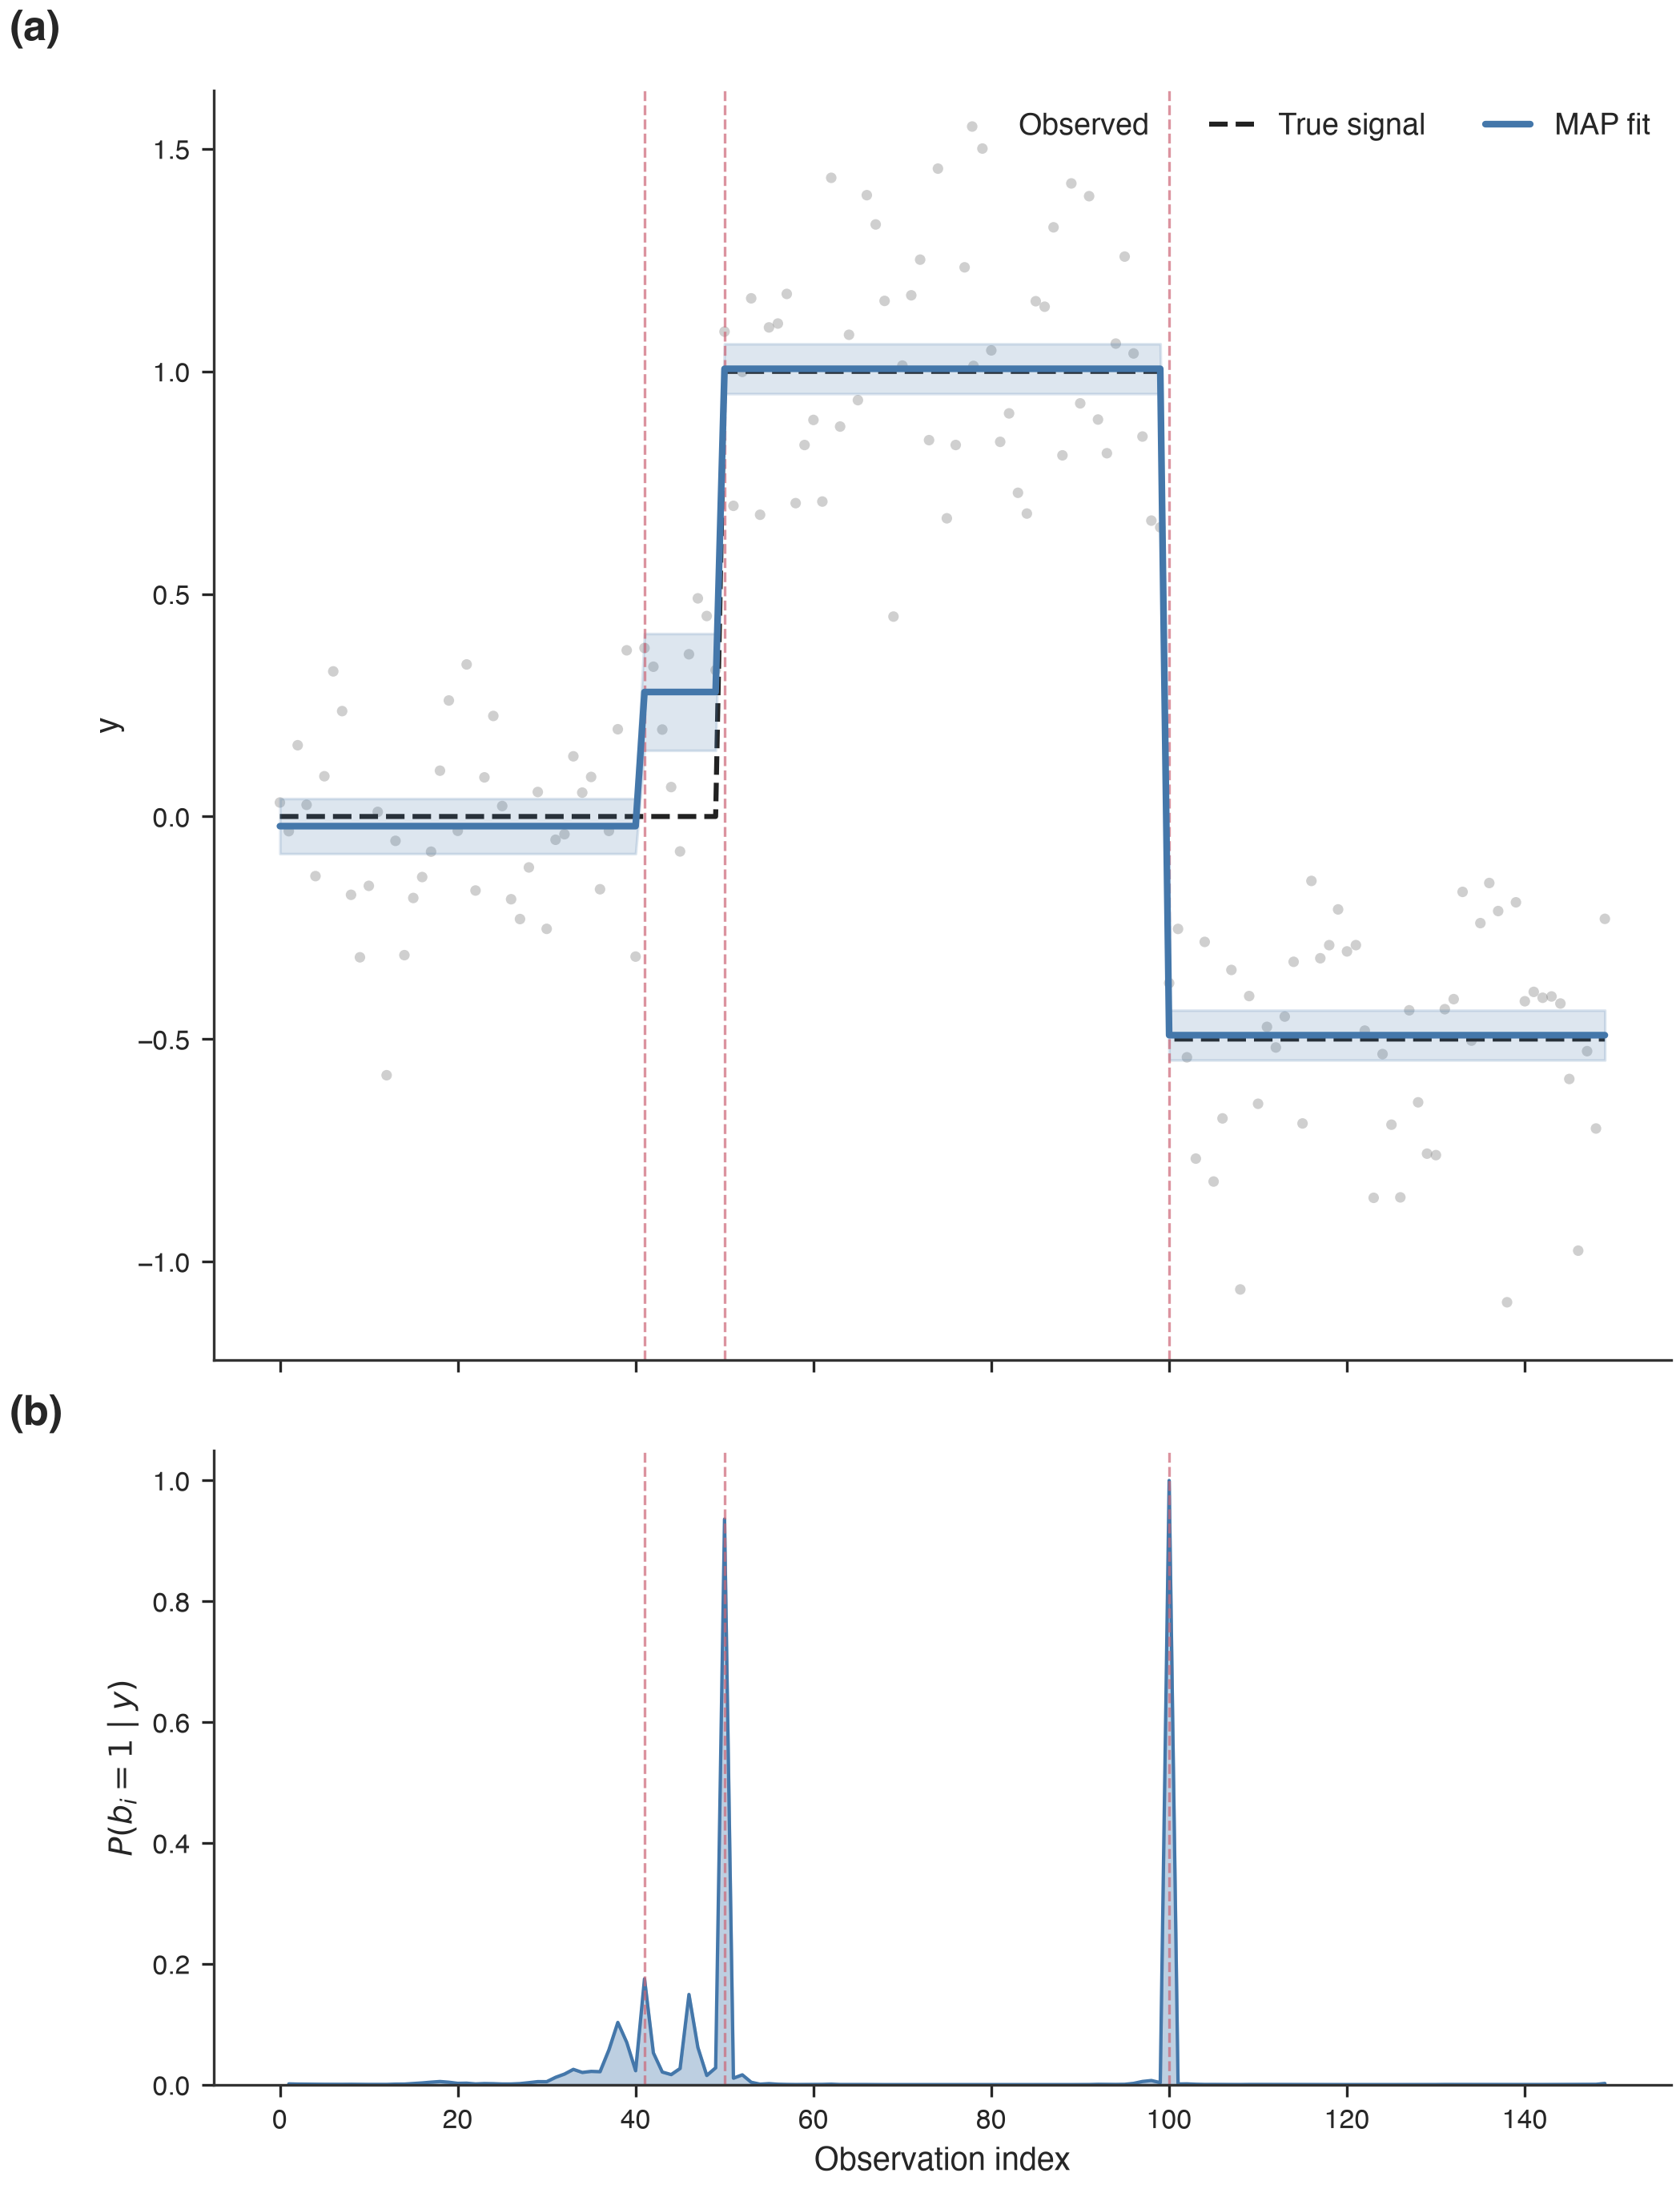
\includegraphics[width=0.94\textwidth,height=0.67\textheight,keepaspectratio]{paper/figures/fig1_synthetic_gaussian.png}
  \caption{Gaussian simulation. Top: marginal boundary-event posterior with generating changepoints shown by dashed lines. Bottom: observations, latent signal, joint-MAP segmentation, and 90\% segment-level posterior intervals.}
  \label{fig:gaussian-result-paper}
\end{figure}


\begin{table}[!htbp]
\centering
\small
\begin{tabular}{lr}\toprule
Quantity & Value\\\midrule
Selected $k$ (\texttt{k\_ml\_}) & 4\\
Posterior mean $\mathbb{E}[k]$ & 4.087\\
MAP $k$ & 4\\
$\log p(y)$ & -18.354\\
\bottomrule\end{tabular}

\caption{Posterior summary for the Gaussian simulation in Figure~\ref{fig:gaussian-result-paper}.}
\label{tab:gaussian-summary-paper}
\end{table}


\FloatBarrier
\subsection{Portability across local observation models}
The same global inference code was applied to Gaussian, Poisson, Binomial, and Beta-valued responses (Figure~\ref{fig:family-result-paper}). Table~\ref{tab:family-result-paper} reports the corresponding synthetic metrics. Gaussian, Binomial, and Beta-valued settings selected the generating three segments; Poisson selected four and had the weakest boundary score and largest reconstruction error in this small benchmark. The result supports interface portability and exposes relative difficulty in the bundled settings; it is not a population-level ranking of families.

\begin{figure}[!htbp]
  \centering
  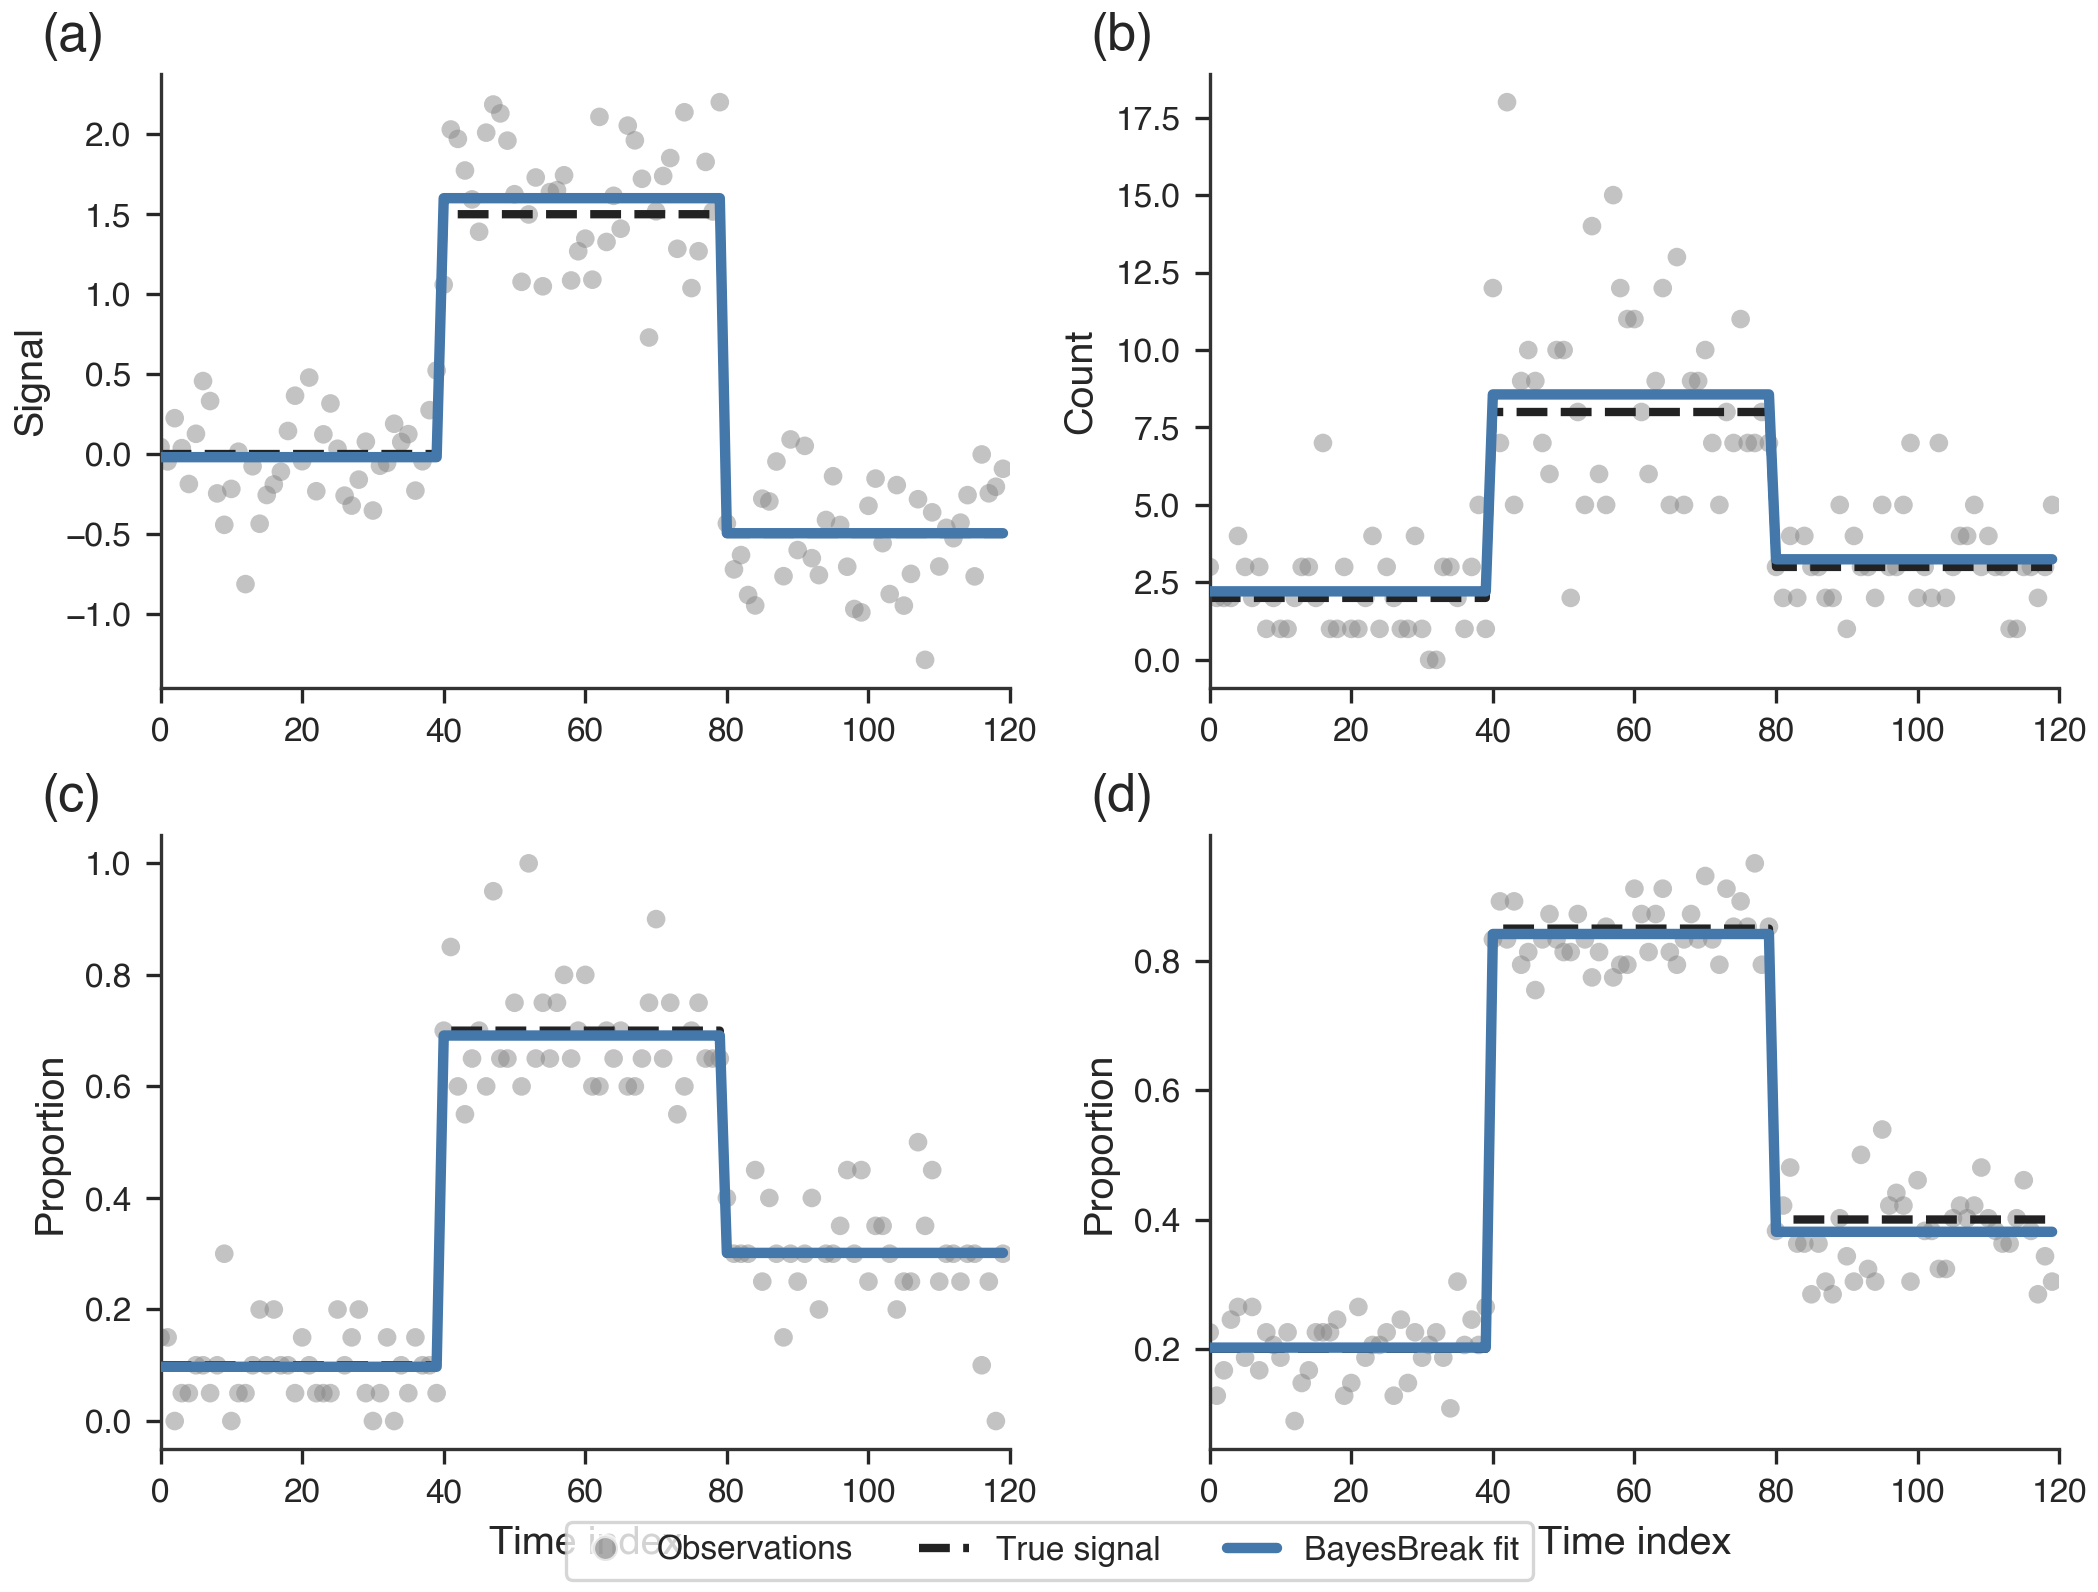
\includegraphics[width=0.95\textwidth,height=0.67\textheight,keepaspectratio]{figures/fig2_family_showcase.png}
  \caption{Observation-family comparison. Gaussian, Poisson, and Binomial use closed-form local conjugate integration; the Beta-valued response uses deterministic one-dimensional quadrature.}
  \label{fig:family-result-paper}
\end{figure}


\begin{table}[!htbp]
\centering
\small
\resizebox{0.88\textwidth}{!}{\begin{tabular}{lrrrrrrr}\toprule
Family & n & $k^\star$ & $\hat{k}$ & F1@$\tau$ & MAE & MSE & $-\log p(y)/n$\\\midrule
Gaussian & 120 & 3 & 3 & 0.992 & 0.00 & 0.0017 & 0.191\\
Poisson & 120 & 3 & 3 & 0.968 & 0.24 & 0.2765 & 2.168\\
Binomial & 120 & 3 & 3 & 1.000 & 0.08 & 0.0004 & 2.109\\
Beta-valued & 120 & 3 & 3 & 1.000 & 0.00 & 0.0001 & 2.619\\
\bottomrule\end{tabular}
}
\caption{Synthetic summary across local observation models. The Beta-valued row is quadrature-based rather than closed-form conjugate.}
\label{tab:family-result-paper}
\end{table}


\FloatBarrier
\subsection{Experiment E00: exactness checks}
\label{sec:e00}
All 380 oracle checks passed (artifact \texttt{03a4d1c38bfe08c1}). Table~\ref{tab:planned-oracles-paper} reports the maximum numerical discrepancy per category. Partition sums and normalizers matched direct partition enumeration to within $1.07\times10^{-14}$ on the log scale across four families (Gaussian, Poisson, Binomial, Negative Binomial) at $n\in\{2,\ldots,10\}$, including nonuniform cohesion and hazard factors. Boundary event marginals and ordered boundary posteriors matched to within $7.11\times10^{-15}$ in absolute probability. First-moment Bayes curves matched to within $7.11\times10^{-15}$ relative error; second-moment Bayes curve comparison with one-dimensional adaptive quadrature had maximum error $6.30\times10^{-7}$, below the declared tolerance of $10^{-6}$. Family-specific block log-evidences matched one-dimensional adaptive quadrature to within $3.91\times10^{-14}$. Maximum discrepancies are consistent with double-precision floating-point rounding. MAP partitions and descriptors matched exactly (error $= 0$) across all cases. No check failed across any family or sequence length.

\subsection{Experiment E02: cross-family recovery}
Experiment E02 evaluated the five declared observation families: Gaussian, Poisson, Binomial, Negative Binomial, and Beta-valued, on a common segmentation design: $k_{\rm true}=3$, exactly equal segment lengths, $n=240$ (conjugate families) or $n=120$ (Beta-obs, quadrature), 100 or 50 independent replicates per cell, two effect magnitudes per family, and the same geometric-decay count prior and $k_{\max}=10$ as E01. Family-specific priors are as declared: $\mu\sim\mathcal{N}(0,4)$ for Gaussian, $\lambda\sim\mathrm{Gamma}(2,1)$ for Poisson, $p\sim\mathrm{Beta}(2,3)$ for Binomial and Negative Binomial, and $\mu\sim\mathrm{Beta}(2,3)$ for Beta-obs. The Negative Binomial dispersion is $r=5$; the segment functional is the count mean $r(1-p)/p$, not $p$.

At the stronger effect setting in each family, F1@3 ranged from $0.88$ (Gaussian, $\Delta=1.5$) to $1.00$ (Beta-obs, $\mu_{\rm mid}=0.8$). At the weaker effect setting, F1@3 ranged from $0.05$ (Gaussian, $\Delta=0.5$) to $0.99$ (Beta-obs, $\mu_{\rm mid}=0.4$). Weak-effect undersegmentation in the Gaussian and Negative Binomial cells ($\mu_{\rm mid}=3$) is again prior-driven: the geometric prior places strong mass on $k<3$ when the likelihood does not decisively separate segments. Binomial and Beta-obs cells showed consistently high recovery even at the lower effect value; this reflects larger effective information per observation when the generating probabilities are well separated from the prior mode. Negative Binomial signal MSE ($0.18$--$0.20$) is substantially larger than in other families, reflecting the higher observation variance of the NegBin model at these parameters. Beta-obs quadrature convergence was confirmed using 128-node Gauss--Legendre quadrature: the maximum Bayes-curve deviation between 128-node and 256-node evaluations was below $5\times10^{-8}$ across both Beta-obs cells and all five oracle replicates, five orders of magnitude below the prespecified $10^{-3}$ gate threshold.

\begin{table}[!htbp]
\centering
\footnotesize
\caption{Observation-family portability. $k_{\rm true}=3$, equal segment lengths, geometric-decay $p(k)$ prior, $k_{\max}=10$. Mean [95\% bootstrap CI] over 100 (conjugate) or 50 (Beta-obs) independent datasets per cell. $\mathrm{F_1}$ at boundary tolerance $\tau=3$.}
\label{tab:E02-recovery-paper}
\begin{tabular}{llccccccc}
\toprule
Family & Param & $n$ & F1@3 & P($k$=3) & Count MAE & Signal MSE & Brier \\
\midrule
Gaussian & $\delta$ & 240 & 0.047 [0.017,0.080] & 0.105 [0.068,0.144] & 1.76 [1.63,1.87] & 0.052 [0.049,0.054] & 0.008 [0.008,0.008] \\
Gaussian & $\delta$ & 240 & 0.880 [0.835,0.920] & 0.748 [0.722,0.771] & 0.03 [0.00,0.07] & 0.029 [0.026,0.032] & 0.006 [0.005,0.006] \\
\midrule
Poisson & $q$ & 240 & 0.354 [0.285,0.429] & 0.494 [0.444,0.543] & 0.53 [0.36,0.71] & 0.093 [0.080,0.105] & 0.008 [0.008,0.008] \\
Poisson & $q$ & 240 & 0.971 [0.948,0.990] & 0.716 [0.694,0.737] & 0.02 [0.00,0.05] & 0.084 [0.073,0.097] & 0.004 [0.004,0.005] \\
\midrule
Binomial & $p_{\mathrm{mid}}$ & 240 & 0.897 [0.851,0.937] & 0.785 [0.760,0.809] & 0.04 [0.01,0.08] & 0.000 [0.000,0.000] & 0.006 [0.005,0.006] \\
Binomial & $p_{\mathrm{mid}}$ & 240 & 0.992 [0.984,0.998] & 0.799 [0.767,0.825] & 0.04 [0.01,0.08] & 0.000 [0.000,0.000] & 0.001 [0.001,0.002] \\
\midrule
NegBin & $\mu_{\mathrm{mid}}$ & 240 & 0.060 [0.030,0.100] & 0.146 [0.097,0.195] & 1.68 [1.53,1.81] & 0.197 [0.186,0.208] & 0.008 [0.008,0.008] \\
NegBin & $\mu_{\mathrm{mid}}$ & 240 & 0.920 [0.880,0.955] & 0.815 [0.802,0.825] & 0.00 [0.00,0.00] & 0.183 [0.159,0.209] & 0.005 [0.005,0.006] \\
\midrule
Beta-obs & $\mu_{\mathrm{mid}}$ & 120 & 0.990 [0.970,1.000] & 0.837 [0.814,0.855] & 0.00 [0.00,0.00] & 0.000 [0.000,0.000] & 0.004 [0.003,0.005] \\
Beta-obs & $\mu_{\mathrm{mid}}$ & 120 & 1.000 [1.000,1.000] & 0.870 [0.851,0.888] & 0.00 [0.00,0.00] & 0.000 [0.000,0.000] & 0.000 [0.000,0.000] \\
\bottomrule
\end{tabular}
\end{table}


\begin{figure}[!htbp]
  \centering
  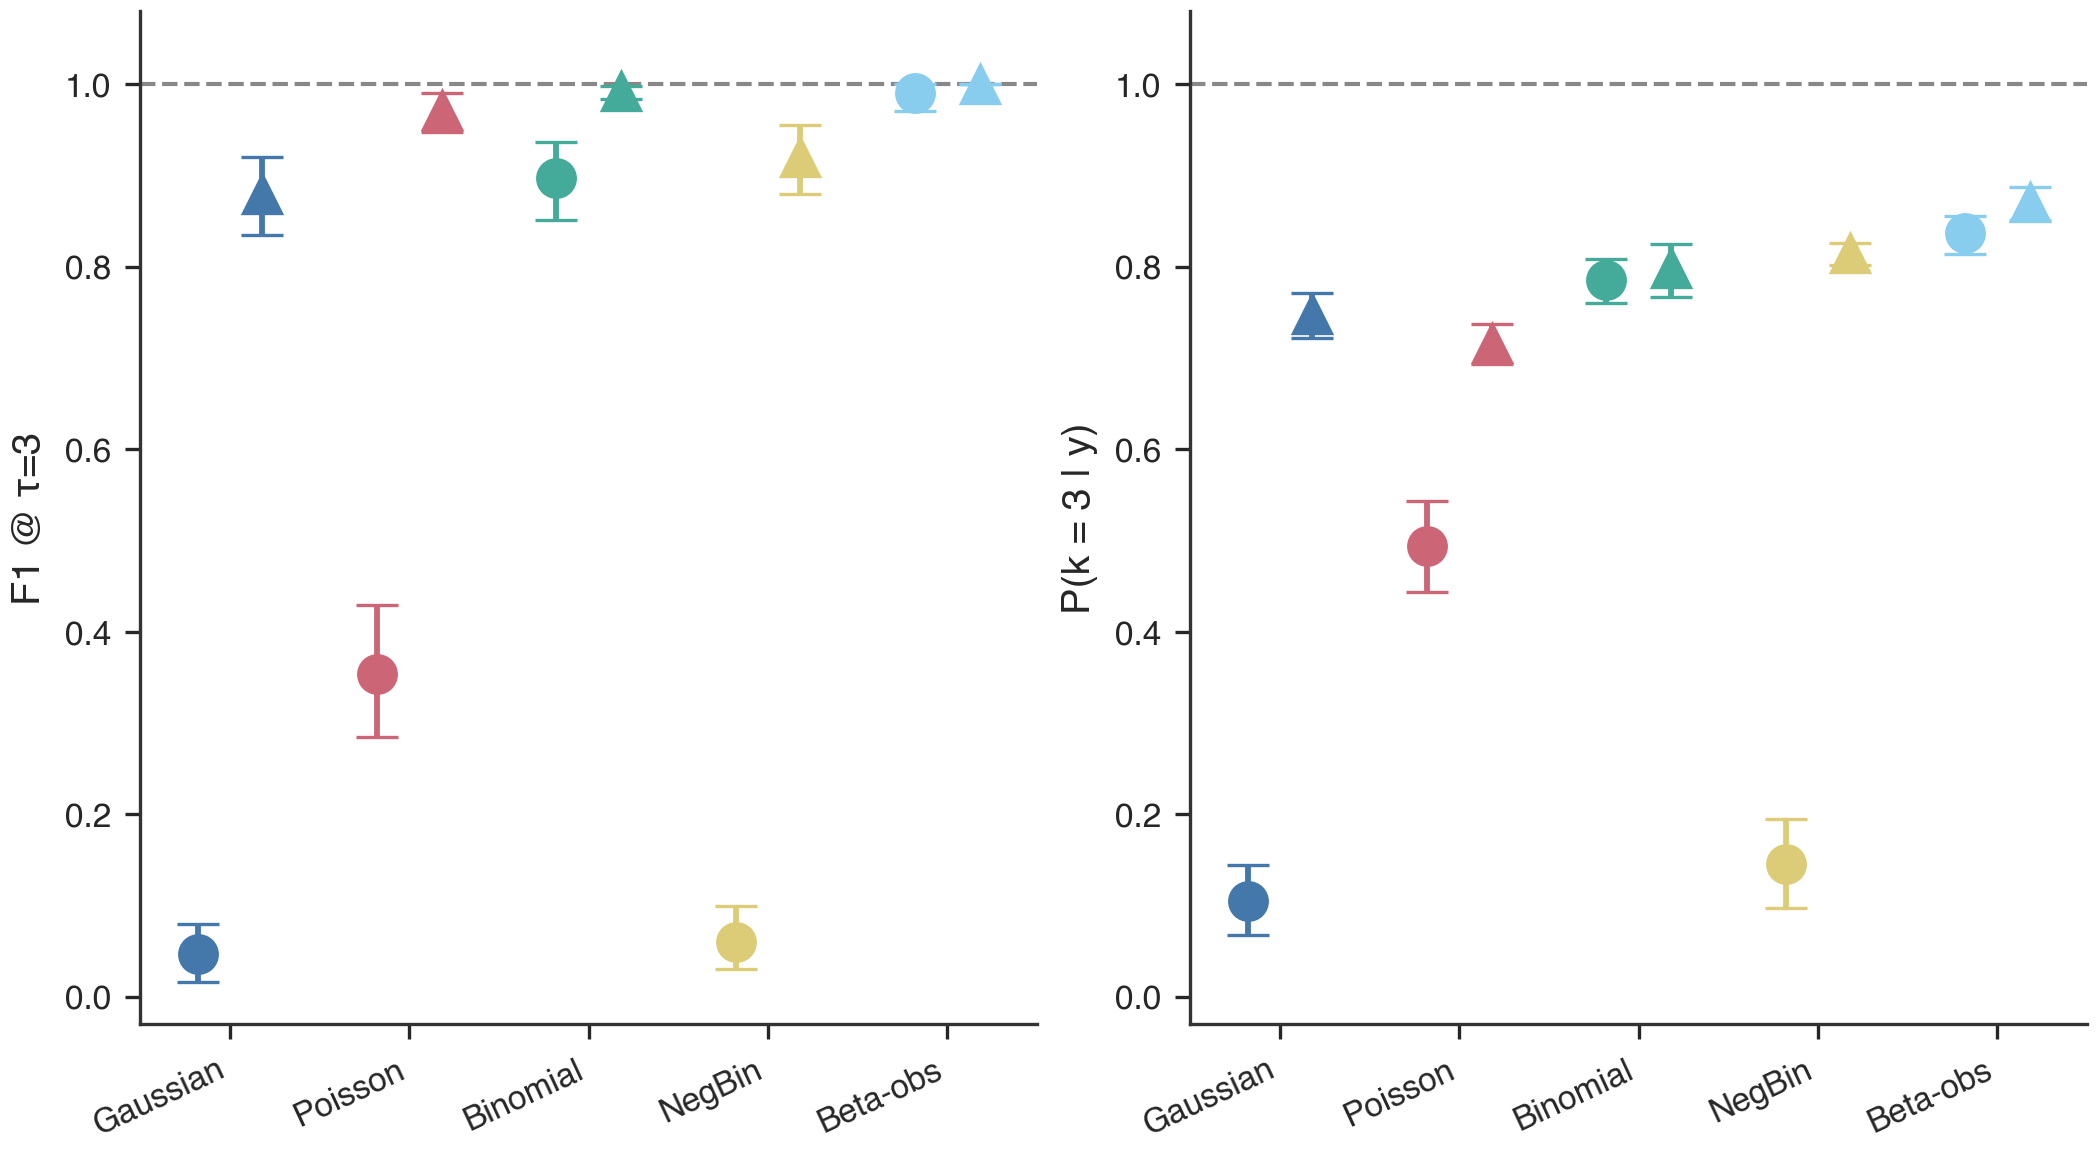
\includegraphics[width=0.97\textwidth,keepaspectratio]{figures/fig_E02_recovery.png}
  \caption{Recovery metrics vs.\ effect magnitude, by observation family. Points are cell means over 100 (conjugate) or 50 (Beta-obs) independent datasets; bands are 95\% bootstrap CIs.}
  \label{fig:E02-recovery-paper}
\end{figure}


Signal MSE is reported on the native family scale and is not directly comparable across families. These results establish mathematical portability of the common inference pipeline across the five declared observation families and expose family-specific difficulty that depends on observation variance and prior placement. They do not establish generalization to other effect sizes, priors, or families not tested in E02.

\FloatBarrier
\subsection{Experiment E03: irregular physical grid and partition prior}
Experiment E03 evaluated four partition priors on Gaussian sequences with an unequal physical spacing at position 120: gap size $G\in\{1,4,16\}$ separates observations $x_{120}$ and $x_{121}$. Two changepoint templates were compared: one with a true changepoint at the gap location (interior boundaries 60,\,120) and one without (interior boundaries 60,\,180). All cells used $n=240$, $\Delta=1.5$, $\sigma=1$, $k_{\max}=8$, and 100 independent replicates. Priors A through D are: A uniform local factors, B gap-proportional boundary hazard, C physical-length cohesion, D the product of B and C. Log-normalizers $C_k$ were computed independently for each prior; the maximum numerical deviation from the brute-force sum was below $10^{-15}$ across all oracle combinations.

Figure~\ref{fig:E03-irregular-paper} shows mean posterior boundary probability $P(b_{120}=1\mid y)$ with 95\% bootstrap bands. When a true changepoint is at the large-gap position, gap hazard prior B raised $P(b_{120}=1\mid y)$ from $0.316$ (uniform, $G=16$) to $0.793$. Combined prior D also increased this probability. When no changepoint is present at the gap (template 60,\,180), all four priors correctly assigned near-zero probability to that position across all gap sizes. Mean F1@3 exceeded $0.85$ in every cell (Table~\ref{tab:planned-E03-prior-paper}), with no prior dominating uniformly across gap sizes and templates. This pattern confirms that prior B and D increase posterior sensitivity at the gap when evidence supports it, without inflating false-positive mass when it does not.

At $G=1$ all physical spacings are equal, so the gap hazard prior is numerically equivalent to uniform; observed differences among the four priors at $G=1$ are sampling variability across independently generated datasets (the four cells use distinct dataset seeds).

\begin{figure}[!htbp]
\centering
\begin{subfigure}[b]{\linewidth}
  \centering
  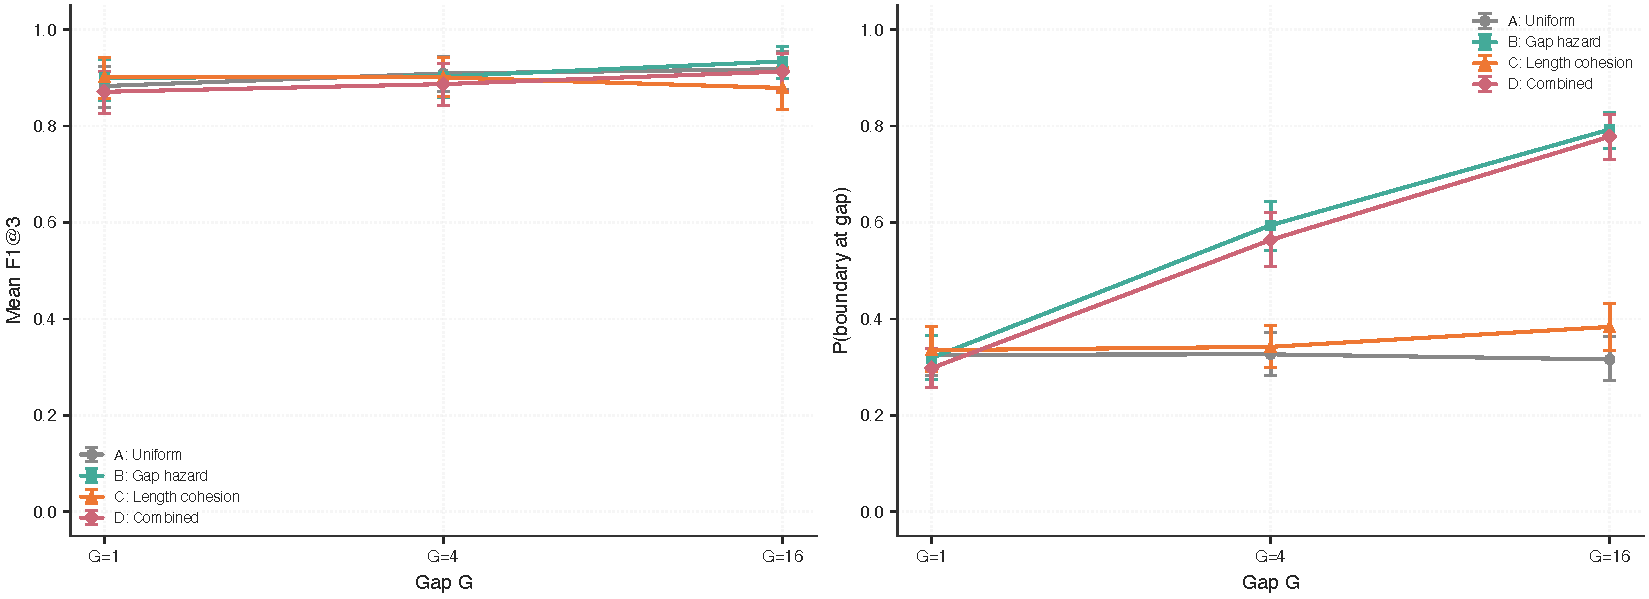
\includegraphics[width=\linewidth]{figures/fig_E03_gap_true.pdf}
  \caption{True changepoint at the gap location ($i=120$). Posterior boundary probability
  increases with gap size $G$ under gap-hazard (B) and combined (D) priors.}
  \label{fig:E03-gap-true-paper}
\end{subfigure}
\vspace{4pt}
\begin{subfigure}[b]{\linewidth}
  \centering
  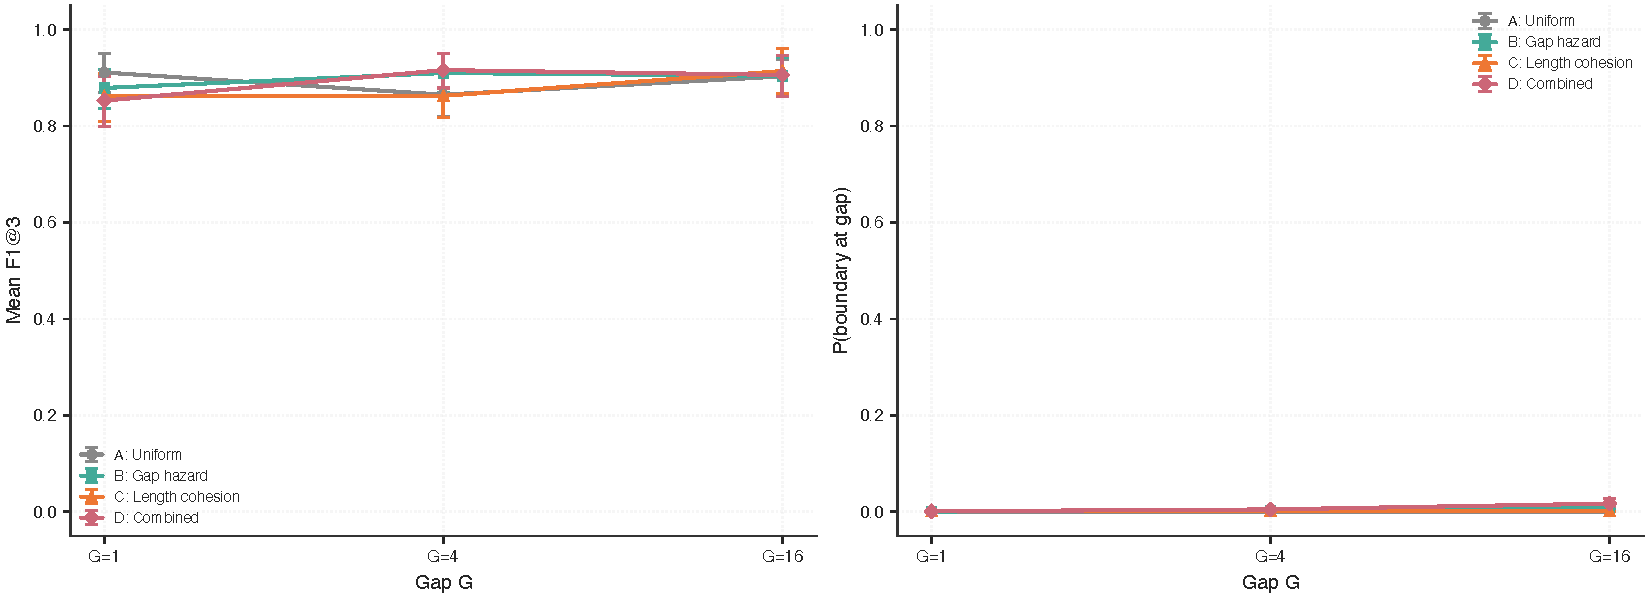
\includegraphics[width=\linewidth]{figures/fig_E03_gap_false.pdf}
  \caption{No changepoint at the gap location. All four priors assign near-zero
  posterior probability at $i=120$ regardless of gap size.}
  \label{fig:E03-gap-false-paper}
\end{subfigure}
\caption{Irregular-design prior ablation. Mean boundary posterior $P(b_{120}=1\mid y)$
with 95\% bootstrap bands across 100 independent datasets. Top panel: generating template
places a true changepoint at the large-gap position (boundaries 60,\,120); gap-hazard
and combined priors correctly raise posterior probability at the gap when evidence
supports a change. Bottom panel: generating template places no changepoint at the gap
(boundaries 60,\,180); all priors correctly preserve near-zero false-positive probability.
Mean $\mathrm{F_1}@3$ exceeds $0.85$ in every cell under all four priors.}
\label{fig:E03-irregular-paper}
\end{figure}


\begin{table}[!htbp]
\centering\small
\caption{Irregular-design prior ablation: mean $\mathrm{F_1}@3$ and $P(b_{120}=1\mid y)$ per cell. 95\% percentile bootstrap intervals from 2000 resamples of independent datasets.}
\label{tab:planned-E03-prior-paper}
\begin{tabular}{@{}llcccc@{}}
\toprule
Gap $G$ & Template & Prior & Mean F1@3 (95\% CI) & $P(b_{120}=1\mid y)$ (95\% CI) & Mean Count Exact \\
\midrule
1 & [60, 120] & A: Uniform & 0.883 [0.839, 0.924] & 0.326 [0.282, 0.366] & 0.980 \\
1 & [60, 120] & B: Gap hazard & 0.900 [0.854, 0.938] & 0.319 [0.274, 0.365] & 0.970 \\
1 & [60, 120] & C: Length cohesion & 0.902 [0.858, 0.943] & 0.335 [0.291, 0.384] & 0.980 \\
1 & [60, 120] & D: Combined & 0.871 [0.826, 0.914] & 0.298 [0.258, 0.340] & 0.980 \\
1 & [60, 180] & A: Uniform & 0.911 [0.869, 0.951] & 0.001 [0.001, 0.001] & 0.980 \\
1 & [60, 180] & B: Gap hazard & 0.879 [0.837, 0.918] & 0.001 [0.000, 0.001] & 0.970 \\
1 & [60, 180] & C: Length cohesion & 0.862 [0.810, 0.908] & 0.001 [0.001, 0.001] & 0.980 \\
1 & [60, 180] & D: Combined & 0.853 [0.799, 0.903] & 0.001 [0.001, 0.002] & 0.960 \\
4 & [60, 120] & A: Uniform & 0.909 [0.872, 0.944] & 0.327 [0.283, 0.372] & 0.970 \\
4 & [60, 120] & B: Gap hazard & 0.903 [0.860, 0.943] & 0.594 [0.542, 0.644] & 0.990 \\
4 & [60, 120] & C: Length cohesion & 0.901 [0.861, 0.943] & 0.342 [0.299, 0.387] & 0.980 \\
4 & [60, 120] & D: Combined & 0.887 [0.843, 0.930] & 0.564 [0.508, 0.620] & 0.970 \\
4 & [60, 180] & A: Uniform & 0.865 [0.820, 0.910] & 0.000 [0.000, 0.001] & 1.000 \\
4 & [60, 180] & B: Gap hazard & 0.910 [0.870, 0.950] & 0.002 [0.002, 0.002] & 1.000 \\
4 & [60, 180] & C: Length cohesion & 0.863 [0.819, 0.910] & 0.001 [0.001, 0.001] & 0.950 \\
4 & [60, 180] & D: Combined & 0.916 [0.879, 0.950] & 0.005 [0.003, 0.007] & 0.970 \\
16 & [60, 120] & A: Uniform & 0.918 [0.876, 0.955] & 0.316 [0.273, 0.364] & 0.980 \\
16 & [60, 120] & B: Gap hazard & 0.934 [0.899, 0.965] & 0.793 [0.753, 0.829] & 0.990 \\
16 & [60, 120] & C: Length cohesion & 0.879 [0.834, 0.922] & 0.384 [0.335, 0.432] & 0.970 \\
16 & [60, 120] & D: Combined & 0.913 [0.871, 0.951] & 0.778 [0.730, 0.824] & 0.990 \\
16 & [60, 180] & A: Uniform & 0.903 [0.864, 0.939] & 0.001 [0.000, 0.001] & 0.990 \\
16 & [60, 180] & B: Gap hazard & 0.904 [0.861, 0.943] & 0.009 [0.006, 0.015] & 0.970 \\
16 & [60, 180] & C: Length cohesion & 0.914 [0.867, 0.960] & 0.001 [0.001, 0.001] & 0.990 \\
16 & [60, 180] & D: Combined & 0.906 [0.861, 0.946] & 0.017 [0.012, 0.027] & 0.980 \\
\bottomrule
\end{tabular}
\end{table}



\FloatBarrier
\subsection{Experiment E04: shared-boundary pooling}
Experiment E04 evaluated exact common-changepoint pooling across $S\in\{1,4,16,64\}$ sequences and nonshared fractions $f\in\{0,0.25,0.5\}$ (12 cells, 100 independent multi-subject datasets per cell). Sequences share true boundaries at (80,\,160); nonshared sequences shift both boundaries by 20 indices. The pooled method fits a single common partition; the independent method fits each sequence separately. Both use $n=240$, $\sigma^2=1$, $\mathcal{N}(0,4)$ segment prior, $k_{\max}=8$, and the geometric-decay count prior.

At full sharing ($f=0$) pooled F1@3 rose from $0.893$ at $S=1$ to $1.000$ at $S\in\{16,64\}$, while independent F1@3 remained near $0.893$ across all $S$ (Figure~\ref{fig:planned-pooled-paper}, Table~\ref{tab:planned-E04-paper}). This confirms the monotone information accumulation property of exact pooling under the common-boundary model. At $f=0.25$ and $f=0.5$, pooled F1@3 degraded substantially for $S\geq4$ because the common-template model is misspecified when some sequences use different boundaries; independent inference was unaffected. The $S=1$, $f=0.5$ cell is a designed boundary case: with one sequence and all boundaries nonshared, pooled and independent inference are equivalent and F1 against the common template is near zero by construction (the recovered boundary at positions 100,\,180 lies 20 indices from the common template, exceeding $\tau=3$). This is not a failure of the estimator; it records the correct behavior of the common-boundary model when given a single sequence with non-template boundaries.

Pooled log evidence and independent per-sequence log evidences arise from different model priors and are not directly comparable as Bayes factors between the pooled and independent models.

\begin{figure}[!htbp]
\centering
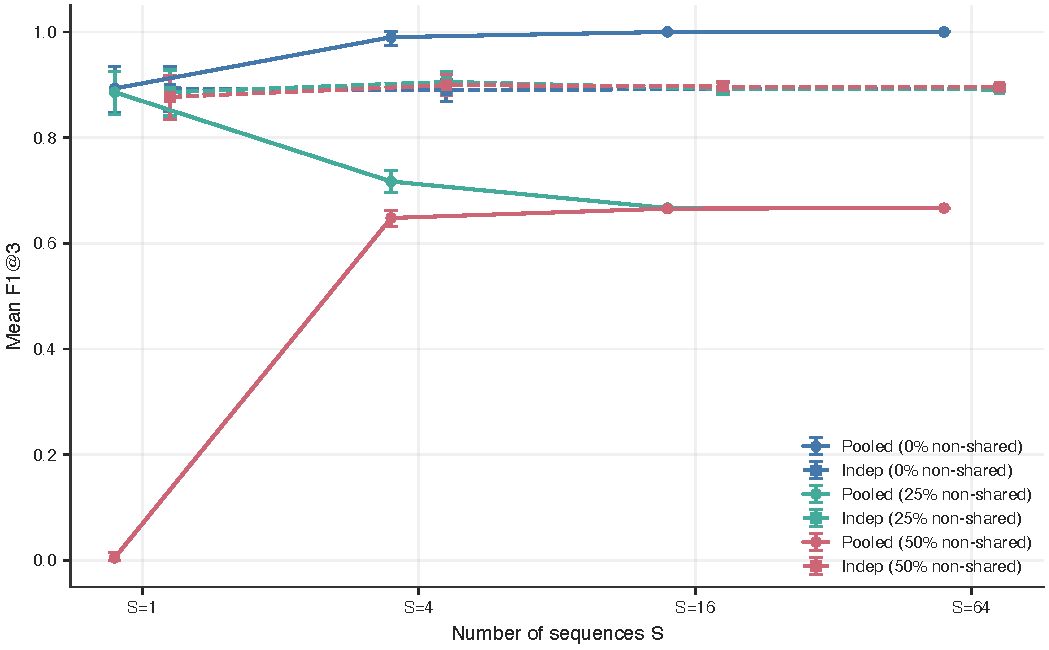
\includegraphics[width=0.92\linewidth]{figures/fig_E04_pooled.pdf}
\caption{Pooled versus independent boundary recovery across number of shared sequences
$S\in\{1,4,16,64\}$ and nonshared fraction $f\in\{0,0.25,0.5\}$.
Pooled F1@3 (solid) and independent per-sequence F1@3 (dashed), with 95\% bootstrap bands.
At full sharing ($f=0$), pooled F1 reaches 1.00 for $S\geq16$ while independent F1 remains
near 0.89 across all $S$. Under partial or complete nonsharing, pooled inference is
misspecified and pooled F1 degrades; independent inference is not affected.
F1 is evaluated against the common template boundaries for the pooled method
and against per-sequence actual boundaries for the independent method.}
\label{fig:planned-pooled-paper}
\end{figure}


\begin{table}[!htbp]
\centering\small
\\caption{Shared-boundary pooling: pooled (SharedBoundary) vs independent (per-sequence) F1@3 and count-exact rate. 95\% percentile bootstrap intervals (2000 resamples, sequence-level).}
\label{tab:planned-E04-paper}
\begin{tabular}{@{}llcccc@{}}
\toprule
$S$ & Nonshared \% & Method & Mean F1@3 (95\% CI) & Count Exact (95\% CI) & Signal MSE (95\% CI) \\
\midrule
1 & 0\% & Pooled & 0.893 [0.847, 0.935] & 0.990 [0.970, 1.000] & 0.035 [0.030, 0.040] \\
1 & 0\% & Independent & 0.893 [0.850, 0.935] & 0.990 [0.970, 1.000] & 0.035 [0.030, 0.041] \\
1 & 25\% & Pooled & 0.886 [0.844, 0.925] & 0.980 [0.950, 1.000] & 0.038 [0.033, 0.043] \\
1 & 25\% & Independent & 0.886 [0.841, 0.928] & 0.980 [0.950, 1.000] & 0.038 [0.033, 0.043] \\
1 & 50\% & Pooled & 0.005 [0.000, 0.015] & 0.960 [0.910, 0.990] & 0.040 [0.034, 0.046] \\
1 & 50\% & Independent & 0.877 [0.834, 0.917] & 0.960 [0.920, 0.990] & 0.040 [0.034, 0.046] \\
4 & 0\% & Pooled & 0.990 [0.975, 1.000] & 1.000 [1.000, 1.000] & 0.017 [0.015, 0.019] \\
4 & 0\% & Independent & 0.890 [0.868, 0.910] & 0.980 [0.965, 0.993] & 0.037 [0.034, 0.040] \\
4 & 25\% & Pooled & 0.717 [0.696, 0.739] & 0.060 [0.020, 0.110] & 0.044 [0.040, 0.048] \\
4 & 25\% & Independent & 0.906 [0.885, 0.925] & 0.975 [0.960, 0.988] & 0.036 [0.033, 0.039] \\
4 & 50\% & Pooled & 0.648 [0.631, 0.663] & 0.000 [0.000, 0.000] & 0.031 [0.028, 0.033] \\
4 & 50\% & Independent & 0.899 [0.879, 0.919] & 0.985 [0.973, 0.995] & 0.036 [0.033, 0.039] \\
16 & 0\% & Pooled & 1.000 [1.000, 1.000] & 1.000 [1.000, 1.000] & 0.013 [0.012, 0.013] \\
16 & 0\% & Independent & 0.892 [0.882, 0.904] & 0.978 [0.971, 0.984] & 0.037 [0.035, 0.038] \\
16 & 25\% & Pooled & 0.667 [0.667, 0.667] & 0.000 [0.000, 0.000] & 0.022 [0.021, 0.023] \\
16 & 25\% & Independent & 0.892 [0.881, 0.904] & 0.973 [0.966, 0.980] & 0.037 [0.035, 0.038] \\
16 & 50\% & Pooled & 0.666 [0.664, 0.667] & 0.000 [0.000, 0.000] & 0.021 [0.020, 0.022] \\
16 & 50\% & Independent & 0.896 [0.887, 0.906] & 0.978 [0.971, 0.985] & 0.037 [0.036, 0.038] \\
64 & 0\% & Pooled & 1.000 [1.000, 1.000] & 1.000 [1.000, 1.000] & 0.012 [0.012, 0.013] \\
64 & 0\% & Independent & 0.893 [0.889, 0.898] & 0.975 [0.971, 0.978] & 0.037 [0.036, 0.038] \\
64 & 25\% & Pooled & 0.667 [0.667, 0.667] & 0.000 [0.000, 0.000] & 0.021 [0.021, 0.021] \\
64 & 25\% & Independent & 0.891 [0.887, 0.896] & 0.973 [0.969, 0.977] & 0.037 [0.037, 0.038] \\
64 & 50\% & Pooled & 0.667 [0.667, 0.667] & 0.000 [0.000, 0.000] & 0.021 [0.021, 0.021] \\
64 & 50\% & Independent & 0.896 [0.890, 0.901] & 0.973 [0.969, 0.977] & 0.037 [0.037, 0.038] \\
\bottomrule
\end{tabular}
\end{table}



\FloatBarrier
\subsection{Calibration and latent-group segmentation}
Experiment E01 evaluated Gaussian segmentation calibration and recovery across 22 predeclared cells (14 primary, 8 prior-ablation), 100 independent replicates per cell, using two sequence lengths ($n\in\{256,512\}$), two true changepoint counts ($k\in\{3,6\}$), three signal-to-noise ratios ($\Delta/\sigma\in\{0.5,1.0,2.0\}$), and two priors. A null cell ($k=1$, $\Delta=0$) verified false-positive control. Boundary-event probabilities are marginalised over $k$ via the full segment-count posterior $p(k\mid y)$.

Reliability diagrams (Figure~\ref{fig:E01-calibration-paper}) showed curves close to the diagonal in every stratum. ECE ranged from $0.00044$ to $0.0081$ across eight pooling strata, with lower ECE at $n=512$ in every matched stratum. Nine of ten equal-mass calibration bins per stratum had mean predicted probability below $0.006$, reflecting correct near-zero assignment to the $\approx97\%$ non-boundary positions; the low aggregate ECE is dominated by accurate null assignment. Mean per-boundary Brier scores ranged from near zero in the null cell to $0.020$ in the $k=6$, $\Delta/\sigma=0.5$, $n=256$ cell (Table~\ref{tab:E01-recovery-paper}).

Recovery under the geometric-decay prior is shown in Figure~\ref{fig:E01-recovery-paper}. At strong signal ($\Delta/\sigma=2$), mean F1@3 exceeded $0.93$ in all primary cells. At weak signal ($\Delta/\sigma=0.5$ with $k=6$), the geometric prior's strong preference for fewer segments caused substantial undersegmentation: 95 of 100 replicates returned modal segment count 1 at $n=256$ and 55 of 100 at $n=512$. This is prior-induced undersegmentation under weak signal. The uniform-prior ablation recovered more boundaries in these cells at the cost of lower P($k$=true) in strong-signal cells. F1@3 improvement with $n$ is consistent but not strictly monotone across all cells. The boundary-position tolerance $\tau=3$ corresponds to $1.2\%$ of sequence length at $n=256$ and $0.6\%$ at $n=512$.

Confidence intervals throughout are 95\% percentile bootstrap intervals from 2000 resamples of independently generated datasets (not boundary positions within a single dataset). Brier and log scores are computed per boundary position marginalized over $k$.

These values support calibration within the generating simulation design. They do not establish robustness to misspecification, performance on non-Gaussian families, or externally validated boundary accuracy.

\textit{Provenance note:} The E01 results directory records SHA256 hashes for all \texttt{src/bayesbreak/} source files. The runner script \texttt{scripts/run\_e01\_gaussian\_calibration.py} was not tracked in git at execution time and its run-time hash cannot be independently verified. A post-execution fingerprint is recorded in \texttt{provenance\_notes.json} under the results directory; complete script-level reproducibility cannot be asserted from the manifest alone.

\begin{figure}[!htbp]
  \centering
  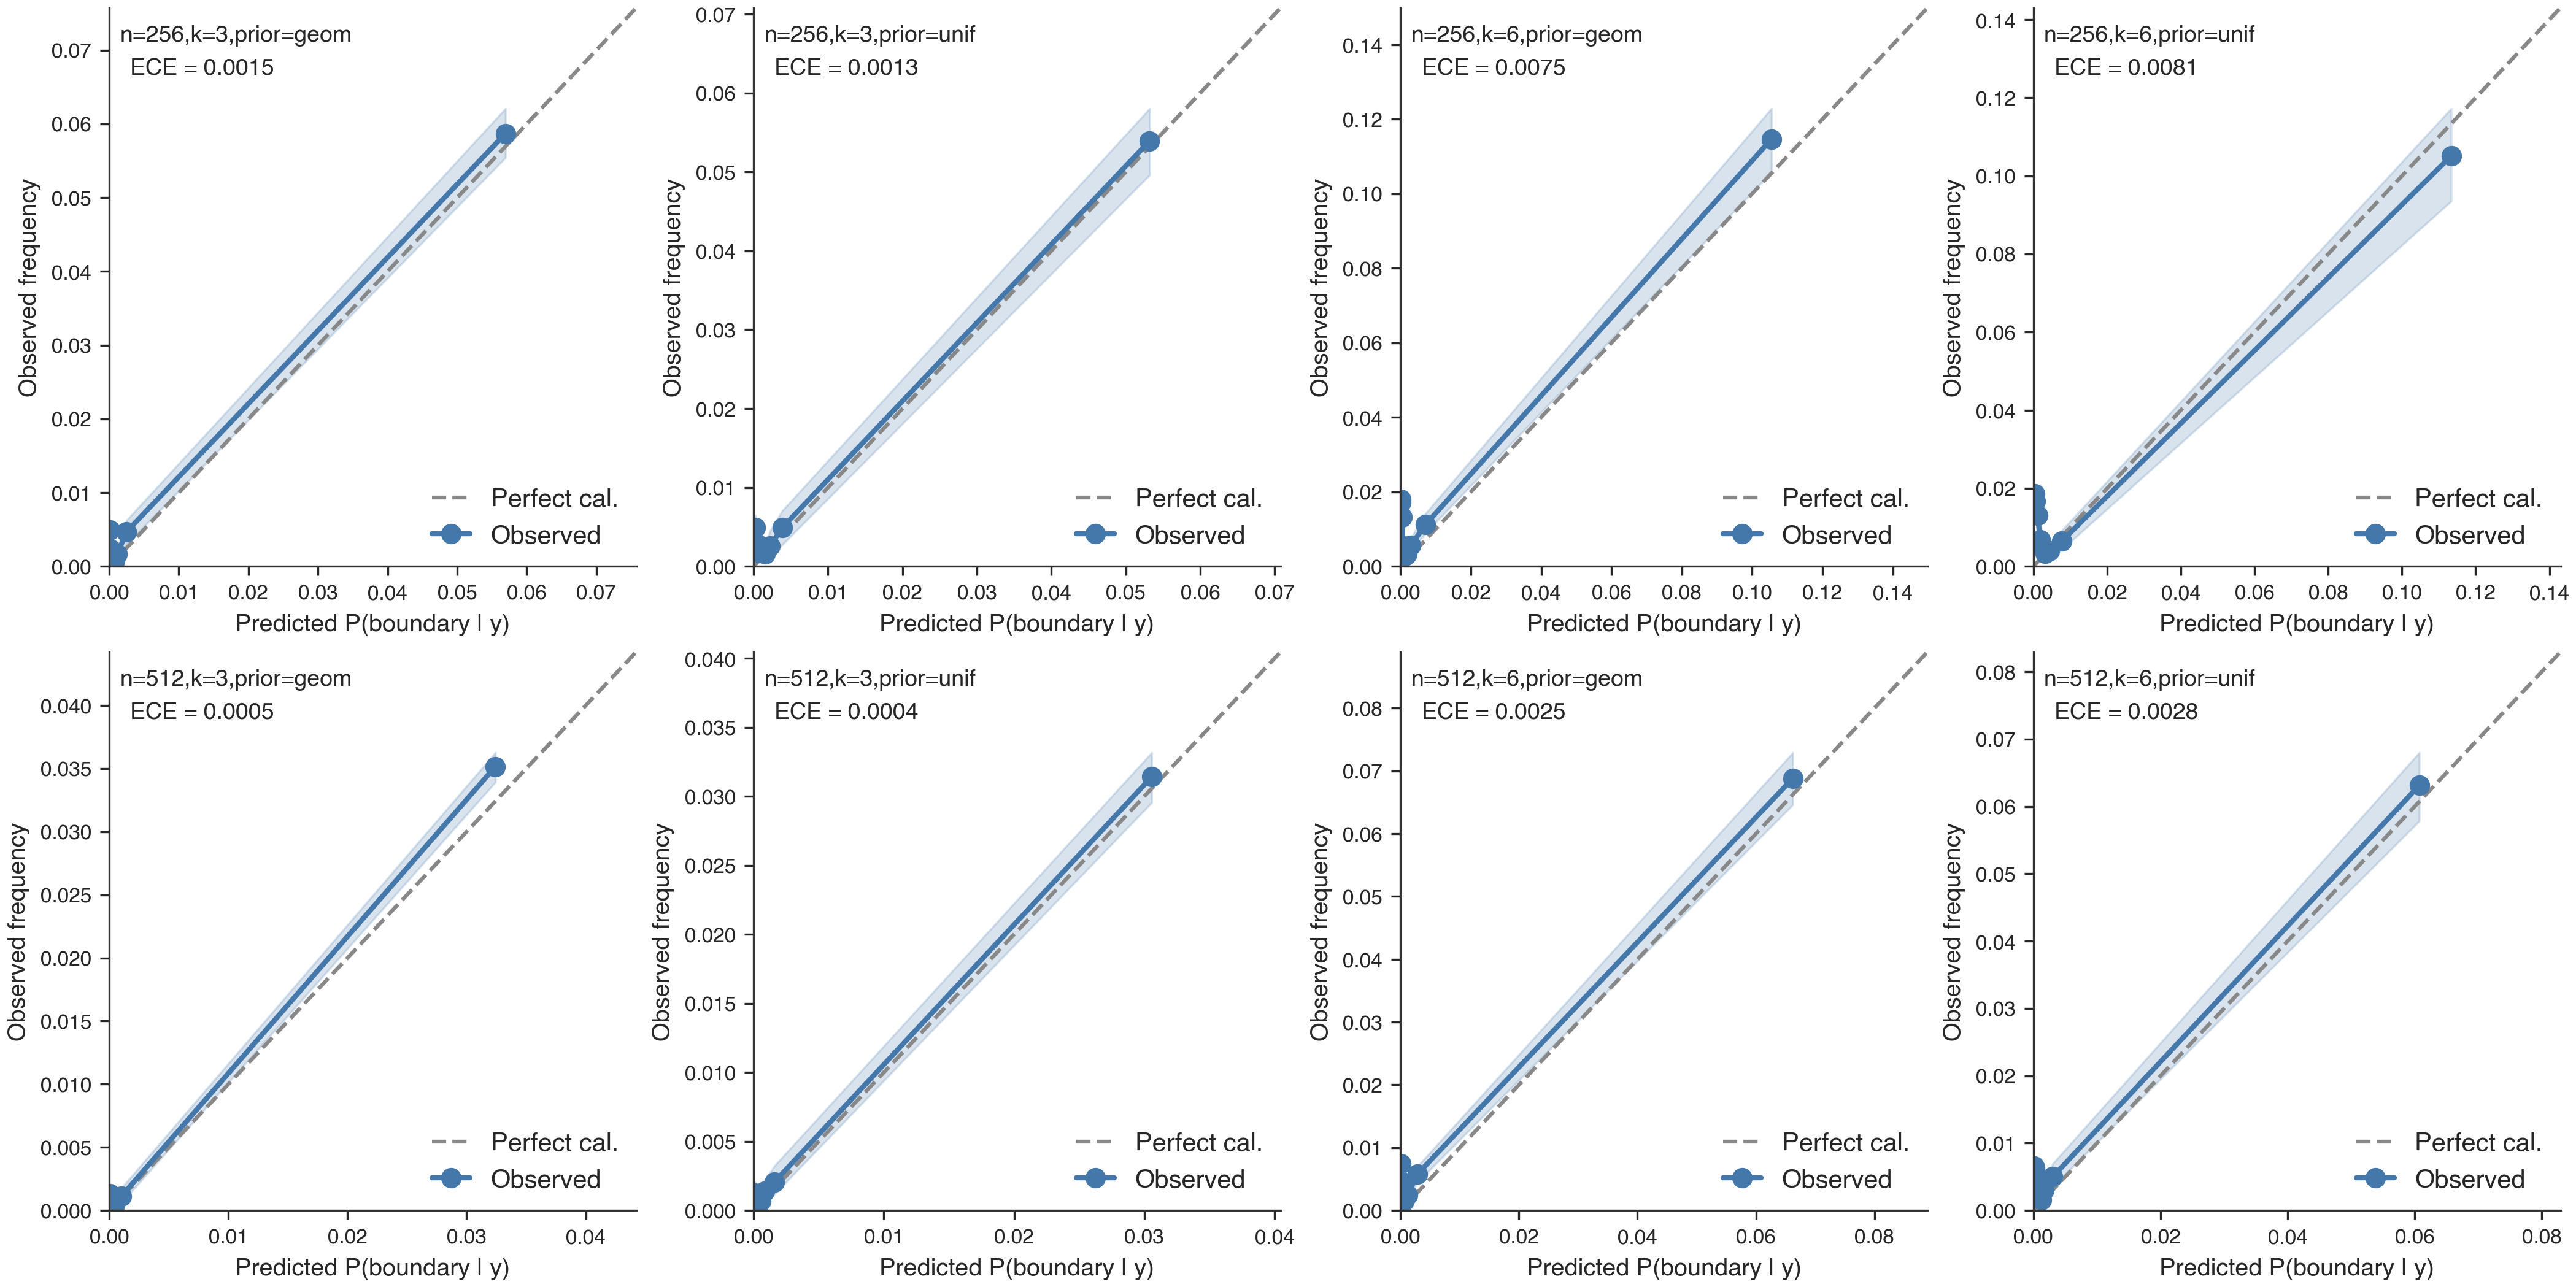
\includegraphics[width=0.97\textwidth,keepaspectratio]{figures/fig_E01_calibration.png}
  \caption{Boundary-event reliability diagrams across pooling strata
    ($n\in\{256,512\}$, $k\in\{3,6\}$, prior $\in\{$geom., unif.$\}$).
    Each panel pools all $\Delta/\sigma$ values within its stratum.
    Bars show equal-mass bin frequencies; shaded bands are 95\% bootstrap confidence intervals
    over 100 replicates; dashed diagonal is perfect calibration.}
  \label{fig:E01-calibration-paper}
\end{figure}


\begin{table}[!htbp]
\centering
\footnotesize
\caption{Gaussian calibration and recovery (primary and prior-ablation cells). Geometric-decay $p(k)$ prior. Mean [95\% bootstrap CI] over 100 independent datasets per cell. $\mathrm{F_1}$ at boundary tolerance $\tau=3$; null cells report expected false-boundary count.}
\label{tab:E01-recovery-paper}
\begin{tabular}{ccccccccc}
\toprule
$n$ & $k_{\rm true}$ & $\Delta/\sigma$ & Prior & F1@3 & P($k$=true) & Count MAE & Brier & Signal MSE \\
\midrule
256 & 1 & 0.0 & Geom. & FP=0.010 & 0.940 [0.922,0.954] & 0.01 [0.00,0.03] & 0.000 [0.000,0.000] & 0.005 [0.004,0.006] \\
256 & 3 & 0.5 & Geom. & 0.083 [0.042,0.130] & 0.120 [0.081,0.165] & 1.69 [1.56,1.82] & 0.008 [0.008,0.008] & 0.043 [0.041,0.046] \\
256 & 3 & 1.0 & Geom. & 0.710 [0.642,0.775] & 0.732 [0.692,0.767] & 0.14 [0.06,0.23] & 0.007 [0.006,0.007] & 0.033 [0.028,0.037] \\
256 & 3 & 2.0 & Geom. & 0.965 [0.935,0.990] & 0.807 [0.792,0.820] & 0.00 [0.00,0.00] & 0.004 [0.003,0.004] & 0.027 [0.024,0.030] \\
256 & 6 & 0.5 & Geom. & 0.009 [0.000,0.024] & 0.000 [0.000,0.000] & 4.94 [4.88,4.99] & 0.020 [0.020,0.020] & 0.063 [0.062,0.064] \\
256 & 6 & 1.0 & Geom. & 0.522 [0.463,0.579] & 0.235 [0.196,0.276] & 1.87 [1.52,2.21] & 0.018 [0.017,0.018] & 0.115 [0.105,0.127] \\
256 & 6 & 2.0 & Geom. & 0.971 [0.955,0.984] & 0.562 [0.538,0.586] & 0.08 [0.03,0.14] & 0.009 [0.009,0.010] & 0.056 [0.051,0.060] \\
\midrule
512 & 1 & 0.0 & Geom. & FP=0.000 & 0.950 [0.938,0.959] & 0.00 [0.00,0.00] & 0.000 [0.000,0.000] & 0.002 [0.001,0.002] \\
512 & 3 & 0.5 & Geom. & 0.203 [0.143,0.267] & 0.353 [0.288,0.420] & 1.06 [0.89,1.24] & 0.004 [0.004,0.004] & 0.025 [0.022,0.028] \\
512 & 3 & 1.0 & Geom. & 0.737 [0.670,0.802] & 0.785 [0.750,0.818] & 0.09 [0.02,0.18] & 0.003 [0.003,0.003] & 0.015 [0.013,0.018] \\
512 & 3 & 2.0 & Geom. & 0.966 [0.939,0.988] & 0.837 [0.817,0.855] & 0.02 [0.00,0.05] & 0.002 [0.002,0.002] & 0.013 [0.012,0.015] \\
512 & 6 & 0.5 & Geom. & 0.078 [0.050,0.108] & 0.006 [0.003,0.011] & 4.34 [4.16,4.51] & 0.010 [0.010,0.010] & 0.050 [0.048,0.052] \\
512 & 6 & 1.0 & Geom. & 0.686 [0.640,0.733] & 0.486 [0.440,0.530] & 0.52 [0.35,0.71] & 0.008 [0.008,0.009] & 0.042 [0.038,0.046] \\
512 & 6 & 2.0 & Geom. & 0.967 [0.952,0.980] & 0.663 [0.641,0.683] & 0.04 [0.01,0.08] & 0.005 [0.005,0.005] & 0.029 [0.026,0.031] \\
\bottomrule
\end{tabular}
\end{table}


\begin{figure}[!htbp]
  \centering
  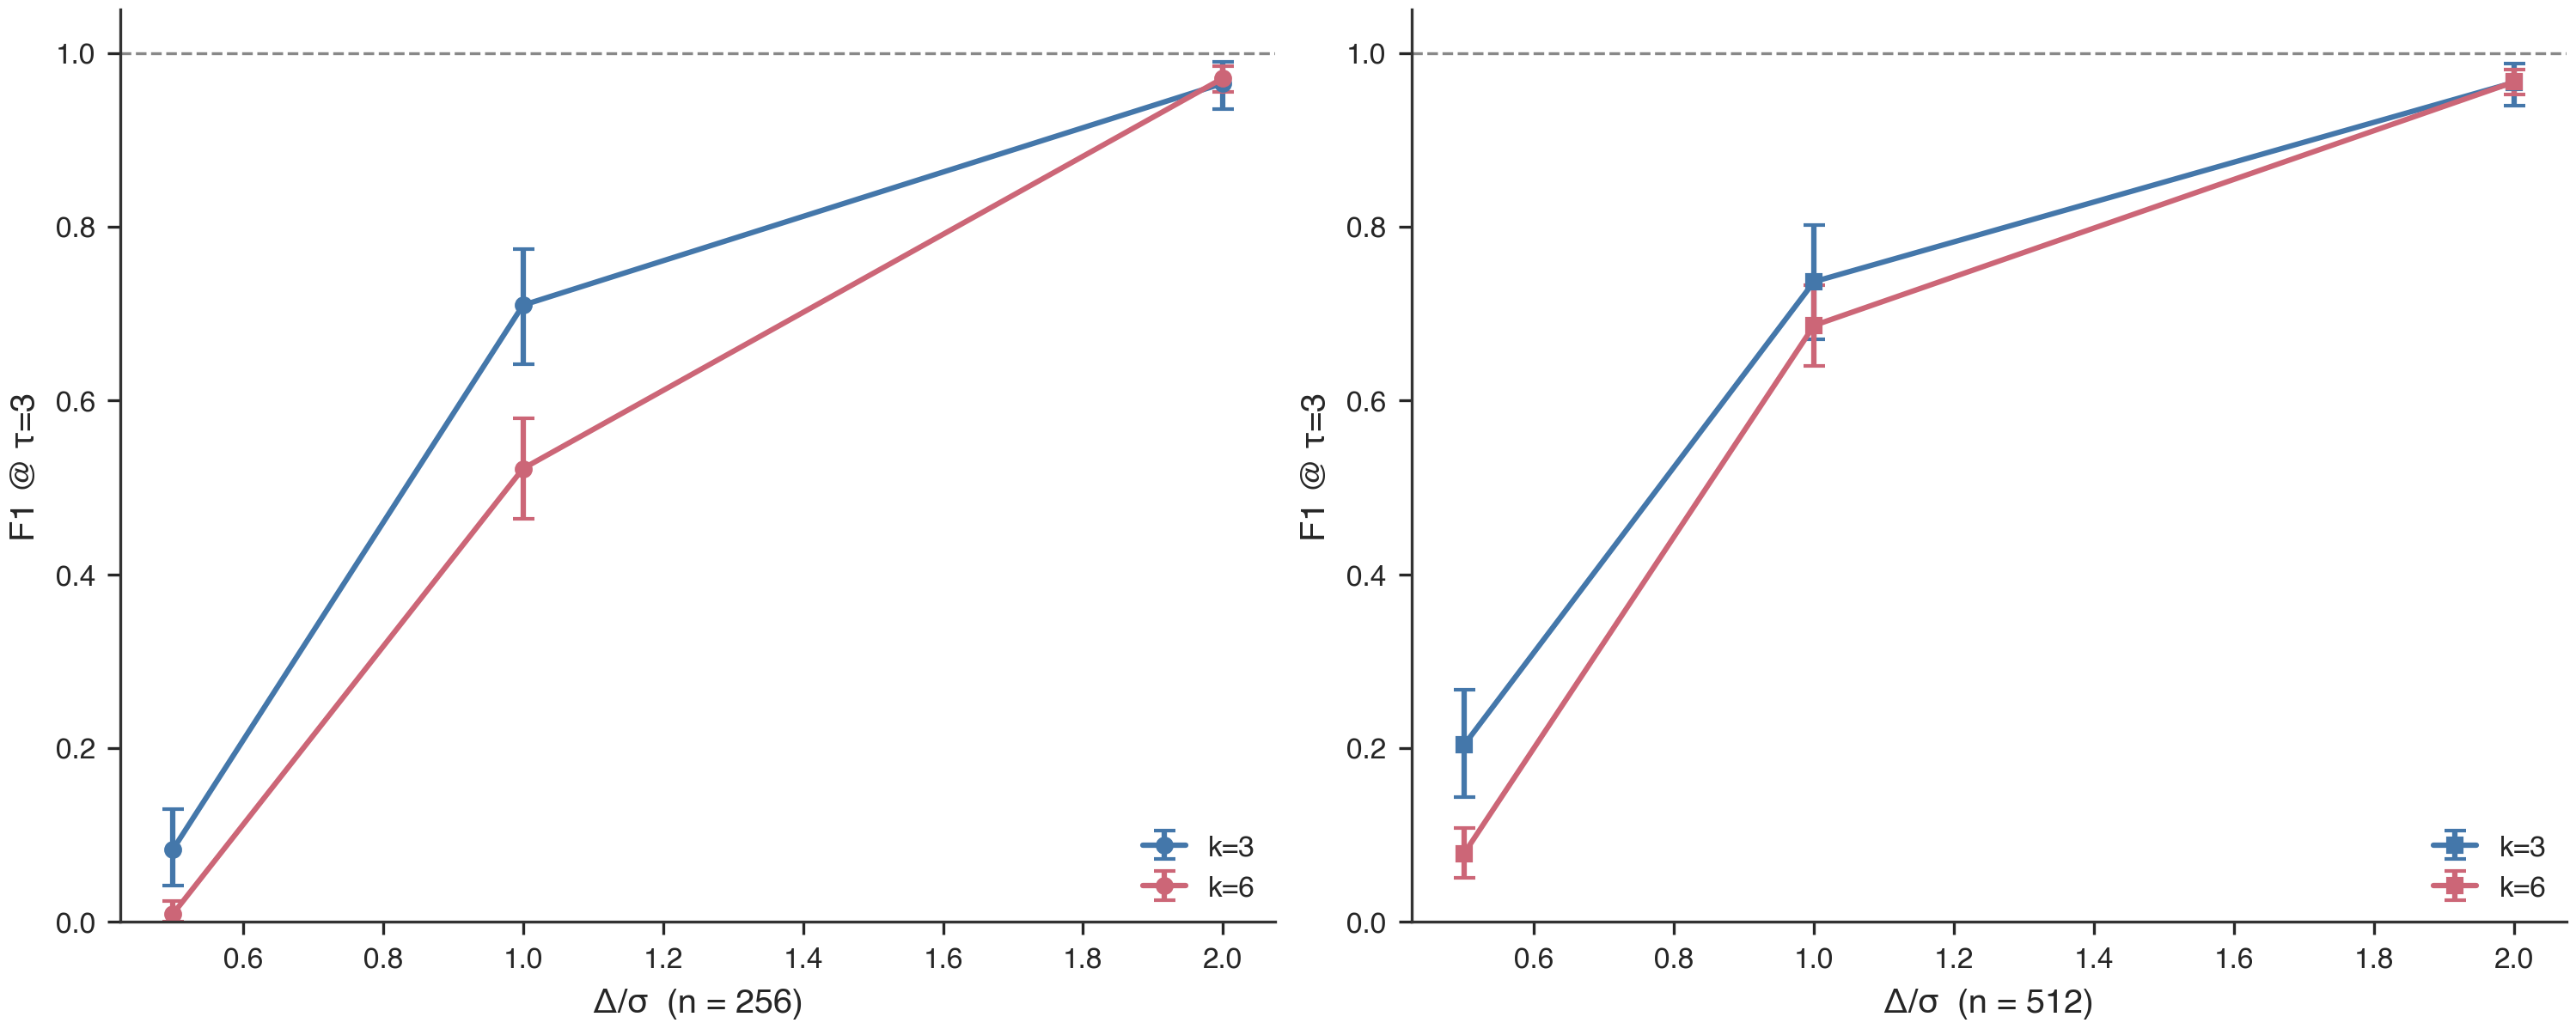
\includegraphics[width=0.97\textwidth,keepaspectratio]{figures/fig_E01_recovery.png}
  \caption{Boundary recovery metrics vs.\ signal-to-noise ratio $\Delta/\sigma$.
    Solid lines: geometric-decay prior; dashed: uniform-prior ablation.
    Points are cell means over 100 replicates; bands are 95\% bootstrap CIs.}
  \label{fig:E01-recovery-paper}
\end{figure}


The latent-group experiment used 24 sequences of length 80 from two known synthetic groups at noise standard deviation $1.0$. It achieved 96\% hard assignment accuracy, with one misassignment and visible ambiguity around the class boundary (Figure~\ref{fig:latent-groups-paper}). Group-specific boundary marginals concentrate near the generating templates. The result is evidence for the finite score-clustering objective in Equation~\eqref{eq:latent-group-objective}; it is not evidence for normalized-mixture identifiability.

\begin{figure}[!htbp]
  \centering
  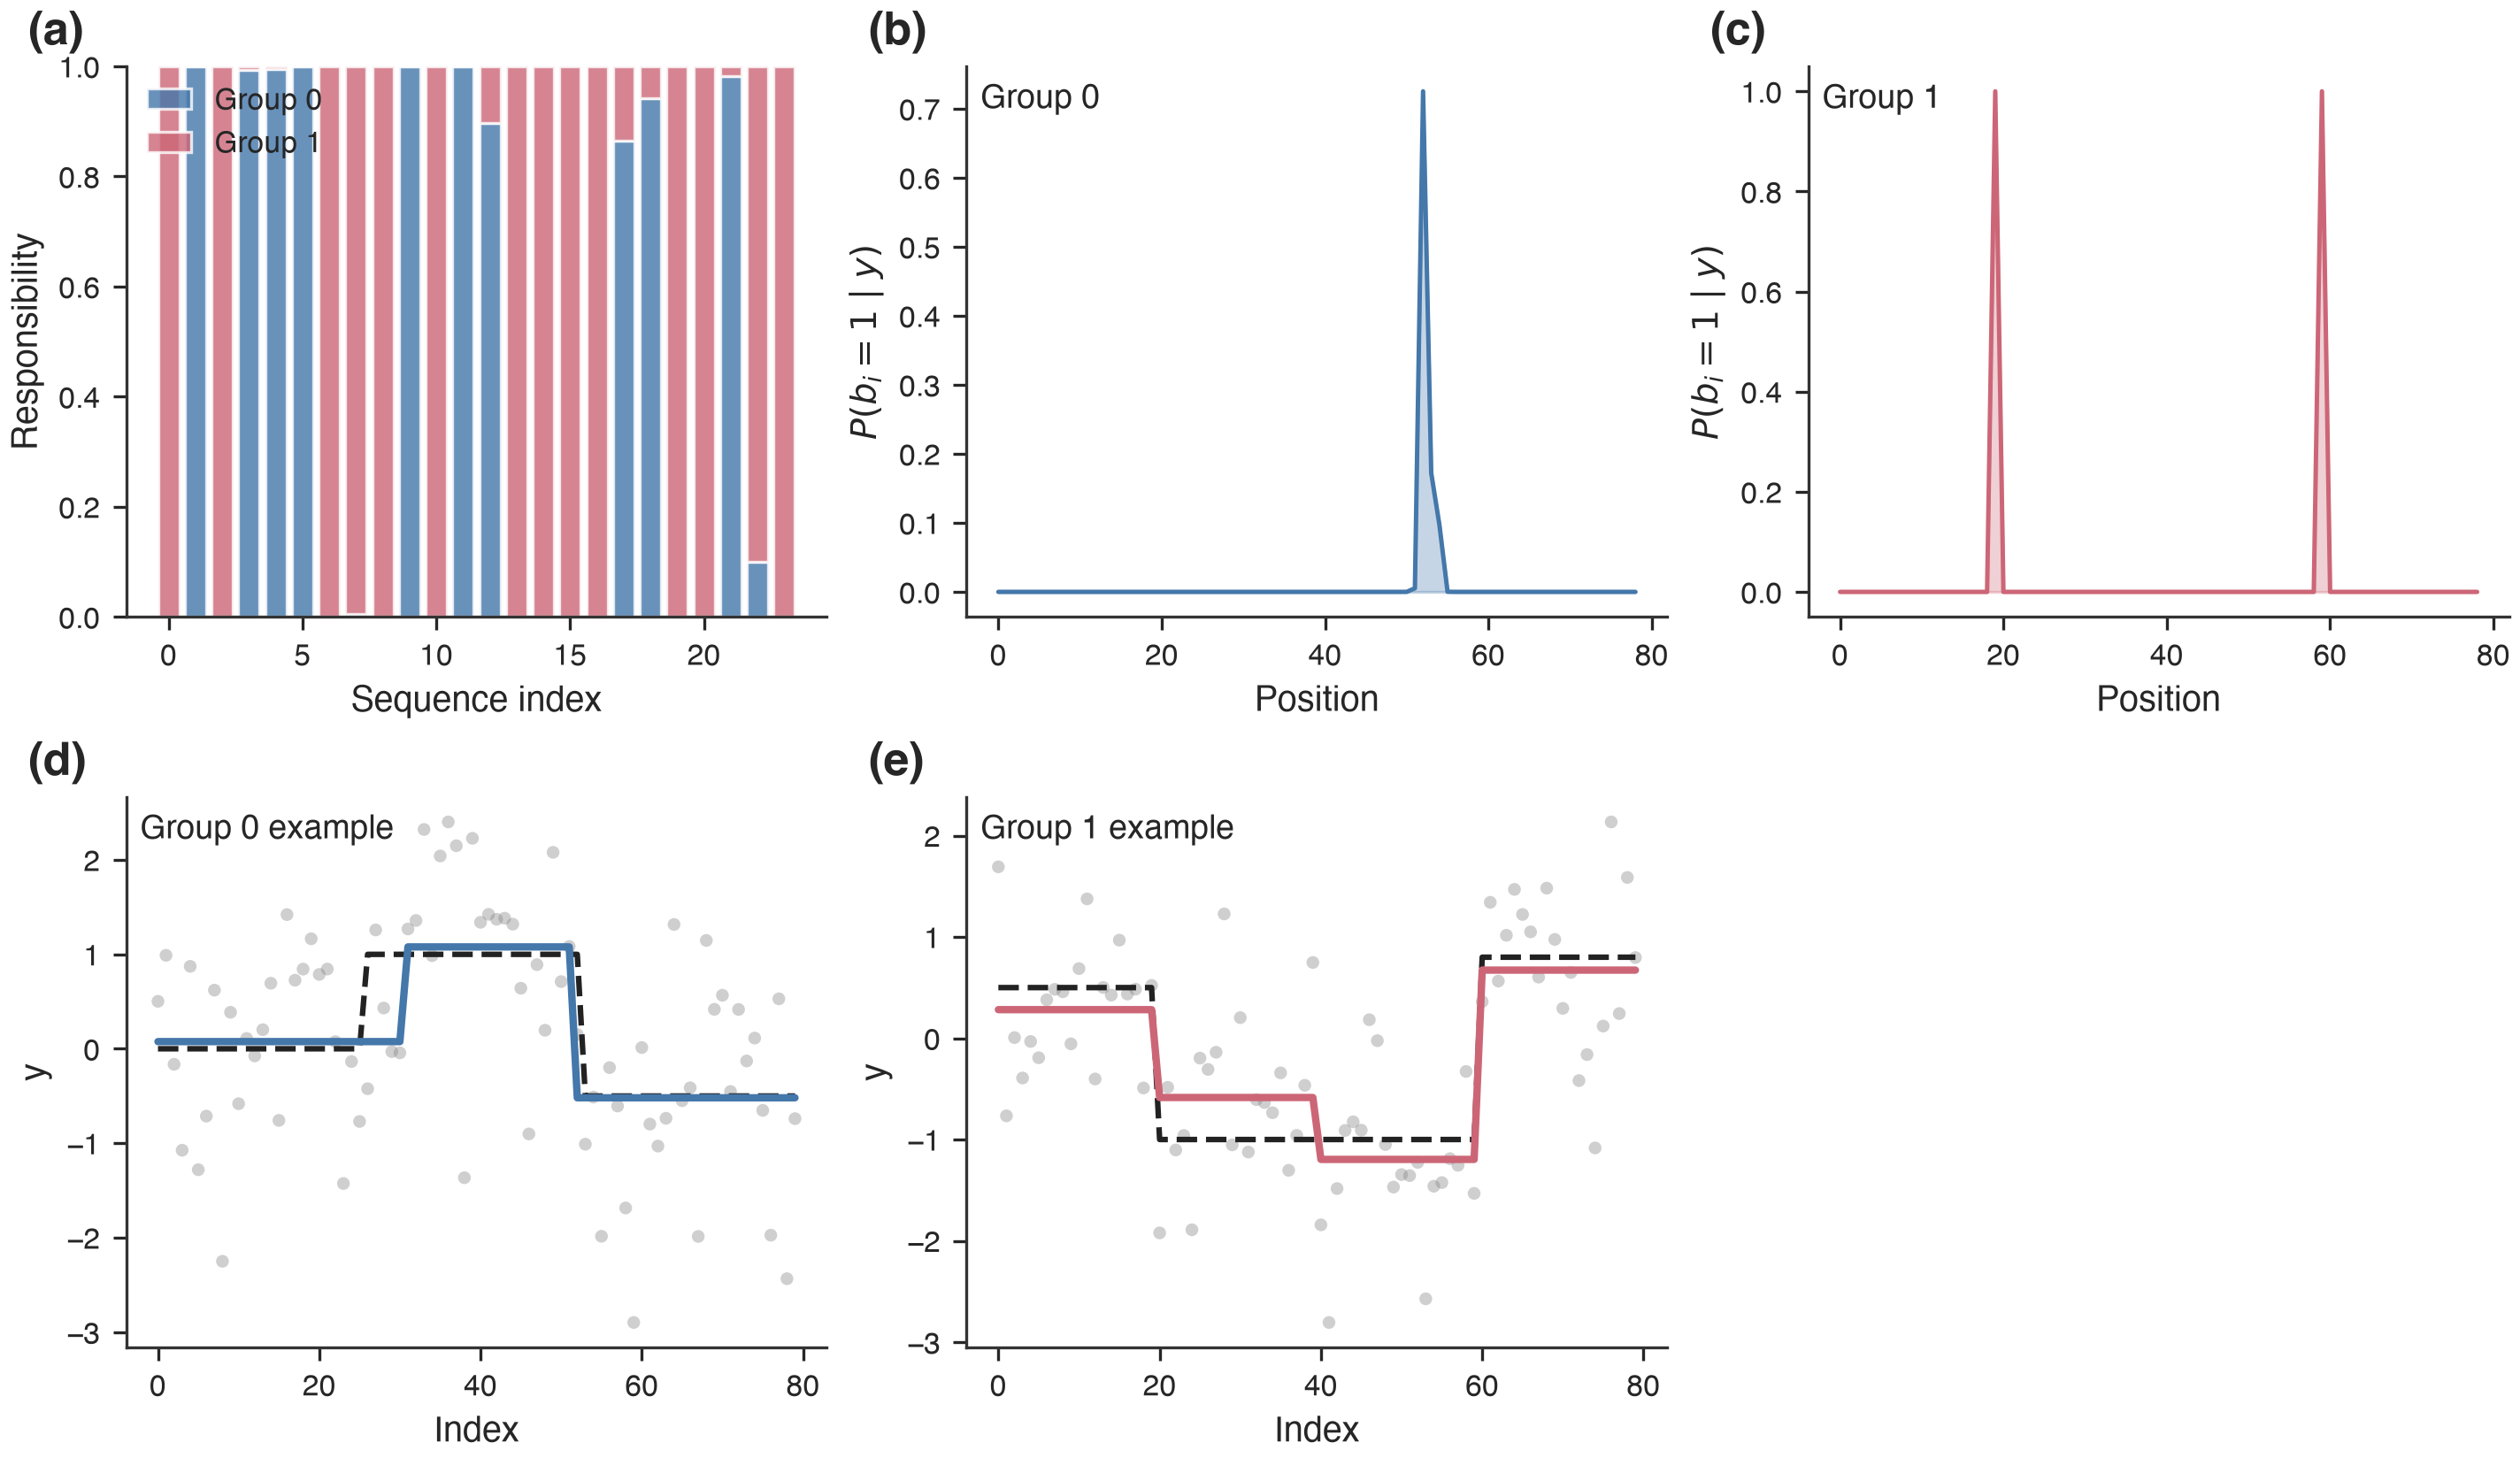
\includegraphics[width=0.97\textwidth,height=0.67\textheight,keepaspectratio]{paper/figures/fig4_latent_groups_cropped.png}
  \caption{Latent-group assignments and group-specific boundary marginals.
    96\% hard recovery for the declared two-template synthetic setting.}
  \label{fig:latent-groups-paper}
\end{figure}


A separate stress study evaluated 400 seeded datasets across eight predeclared cells. In the reference simulation cell, mean label-invariant hard accuracy was $0.9742$ (95\% interval $0.9536$--$0.9948$) and mean adjusted Rand index was $0.9183$. All 400 objective traces were monotone, every returned final objective equaled the final trace value, and all 1,200 restarts were valid. Recovery degraded under low separation, duplicate templates, higher noise, and shorter sequences, as summarized in Figure~\ref{fig:latent-stress-corrected-paper}. These results support the finite score-clustering criterion in the declared simulations, not normalized-mixture identifiability.

\begin{figure}[!htbp]
  \centering
  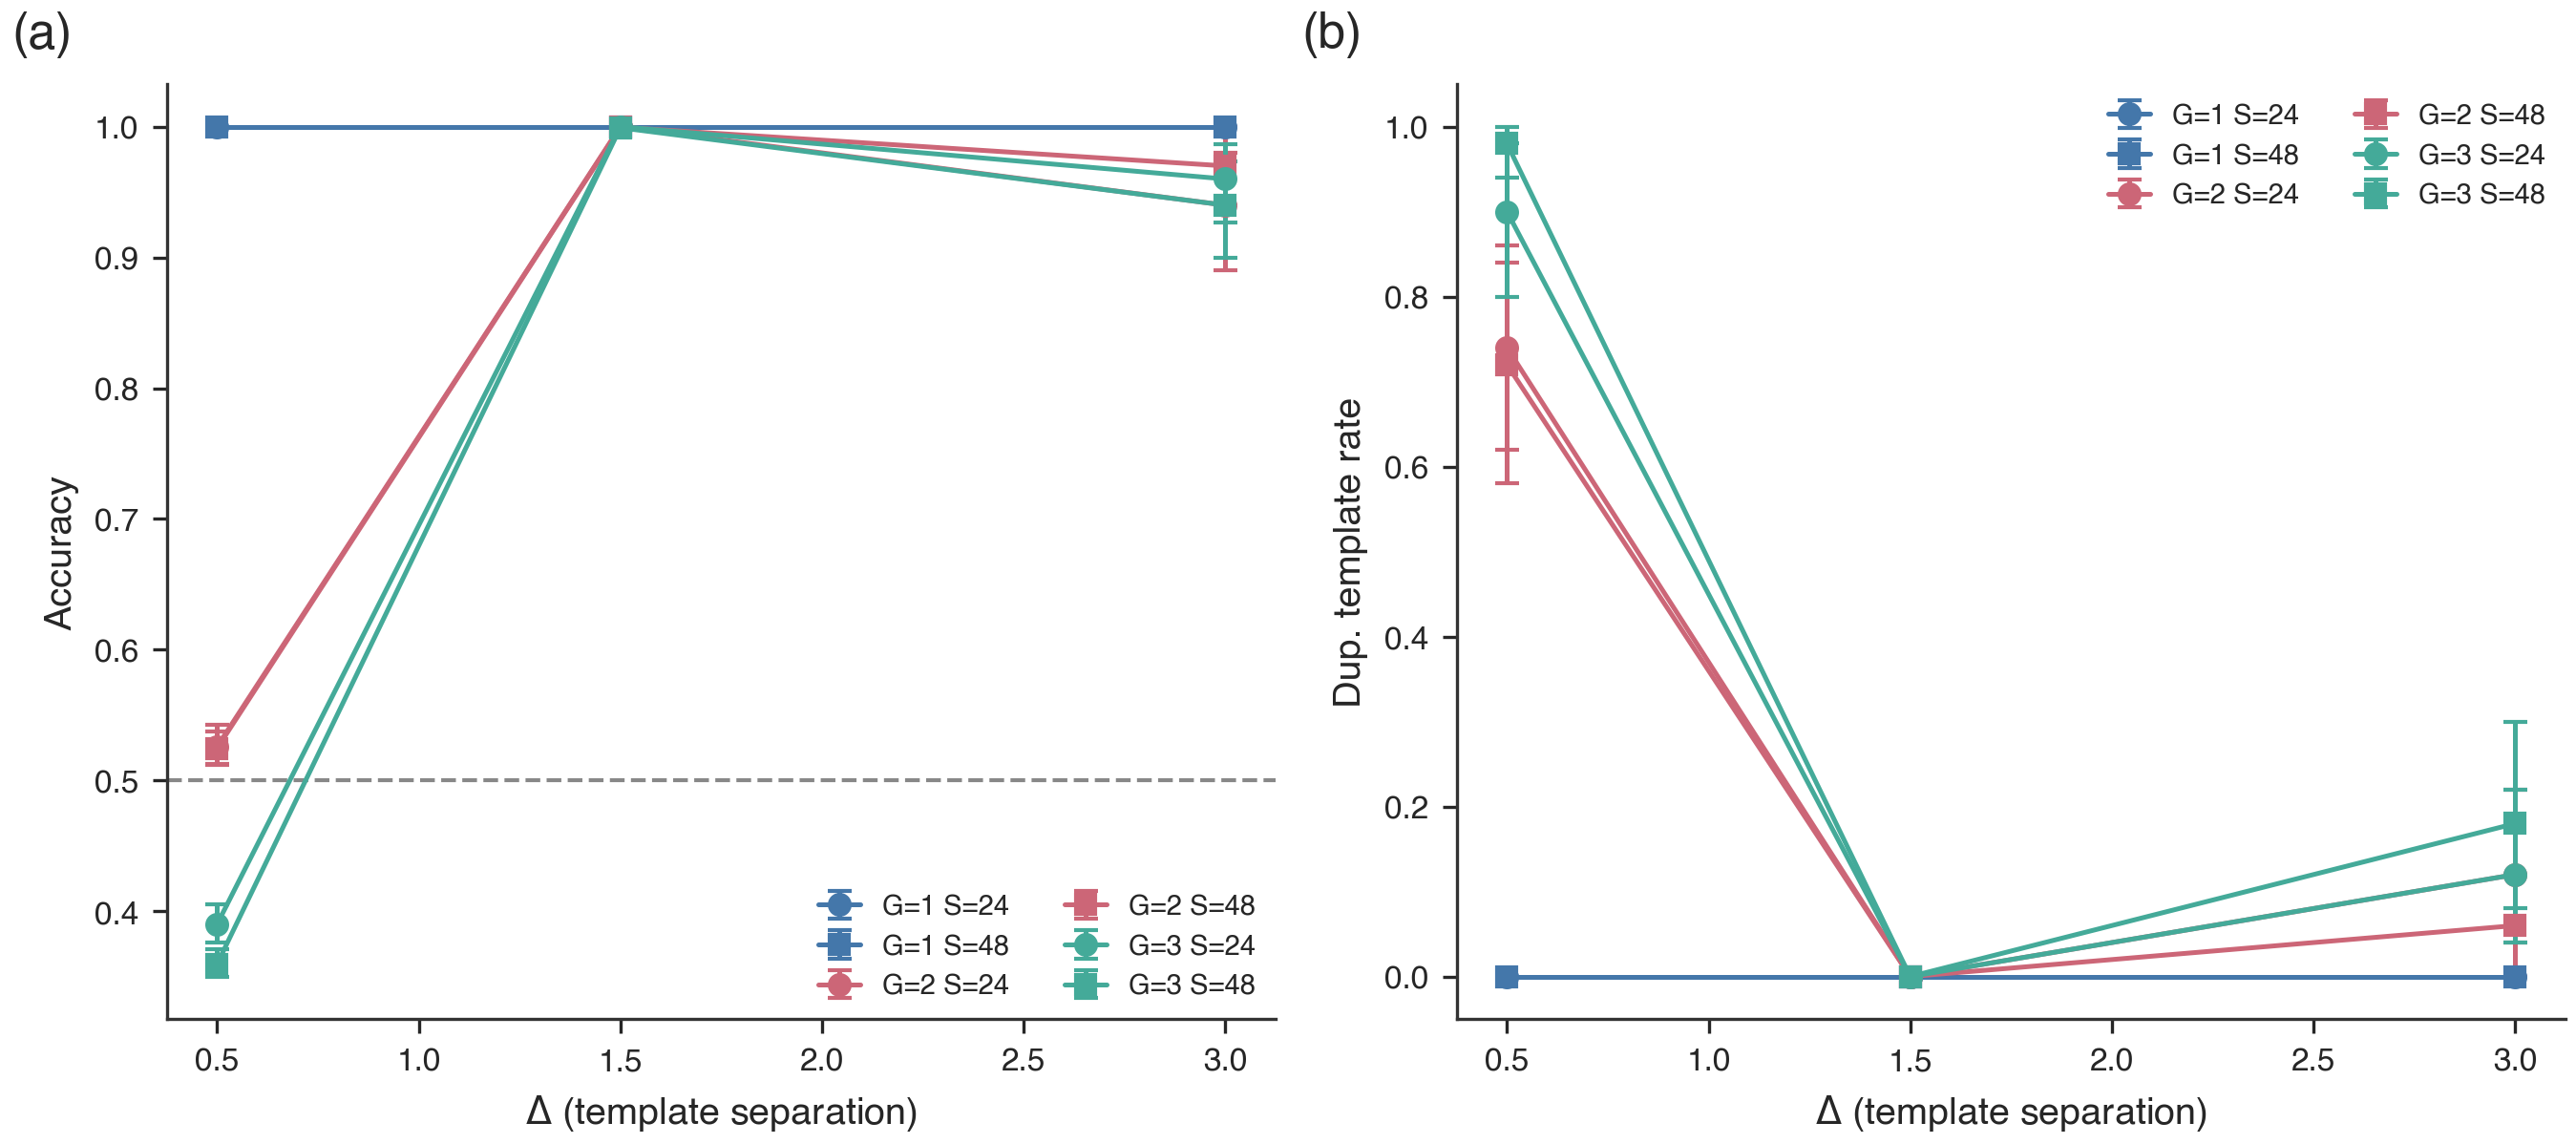
\includegraphics[width=0.88\textwidth]{figures/fig_latent_template_stress.png}
  \caption{Latent-group stress study.
    Top: label-invariant hard accuracy with dataset-level 95\% intervals.
    Bottom: collapsed or duplicate-template rate.
    The dashed $0.5$ line is a descriptive reference, not a universal recovery threshold.}
  \label{fig:latent-stress-corrected-paper}
\end{figure}


\FloatBarrier
\subsection{Experiment E05: finite latent-template score clustering}
Experiment E05 evaluated the template-mixture EM on 18 cells: $G\in\{1,2,3\}$ latent groups, $S\in\{24,48\}$ sequences per dataset, and $\Delta\in\{0.5,1.5,3.0\}$, using 50 independently generated datasets per cell and 5 random restarts per dataset. Group templates are (60,\,120), (90,\,150), and (45,\,105); middle-segment means are $(0,\,(-1)^g\Delta,\,0)$ for group $g$, so labels are not separated by boundary position alone. All sequences use $n=180$, $\sigma=1$, $\mathcal{N}(0,4)$ segment prior, $k_{\max}=8$, and the geometric-decay count prior. Per-subject segment means are independently perturbed by $\mathcal{N}(0,0.25^2)$.

At $\Delta=0.5$, group templates collapsed for $G\geq2$: duplicate-template frequency was $0.72$ for $G=2$ and $0.98$ for $G=3$ at $S=48$. Mean accuracy fell to $0.525$ for $G=2$ and $0.360$ for $G=3$, near the chance levels of $0.5$ and $0.333$ respectively. At $\Delta=1.5$ all cells with $G\leq3$ recovered essentially perfectly: mean accuracy reached $1.000$ and ARI reached $1.000$ for $G=2$; for $G=3$ mean accuracy was $1.000$ [1.000,\,1.000] at $S=24$ and $0.999$ [0.998,\,1.000] at $S=48$ (Figure~\ref{fig:planned-templates-paper}, Table~\ref{tab:E05-latent}). At $\Delta=3.0$ accuracy and ARI were high ($0.940$--$0.970$ for $G=2$, $0.940$--$0.960$ for $G=3$) but occasional degenerate local optima with duplicate templates persisted in a minority of replicates ($0.06$--$0.18$ frequency) despite five restarts, consistent with the non-uniqueness of the template-mixture objective established in the theory section.

All 900 objective traces were non-decreasing within the declared absolute tolerance of $10^{-9}(1+|F|)$, confirming monotone ascent of the finite-template score objective. No replicate failed. Duplicate templates at strong signal reflect local-optima sensitivity and are not a calibration failure; the template-mixture objective is not identifiable when $G$ is overspecified.

\begin{figure}[!htbp]
\centering
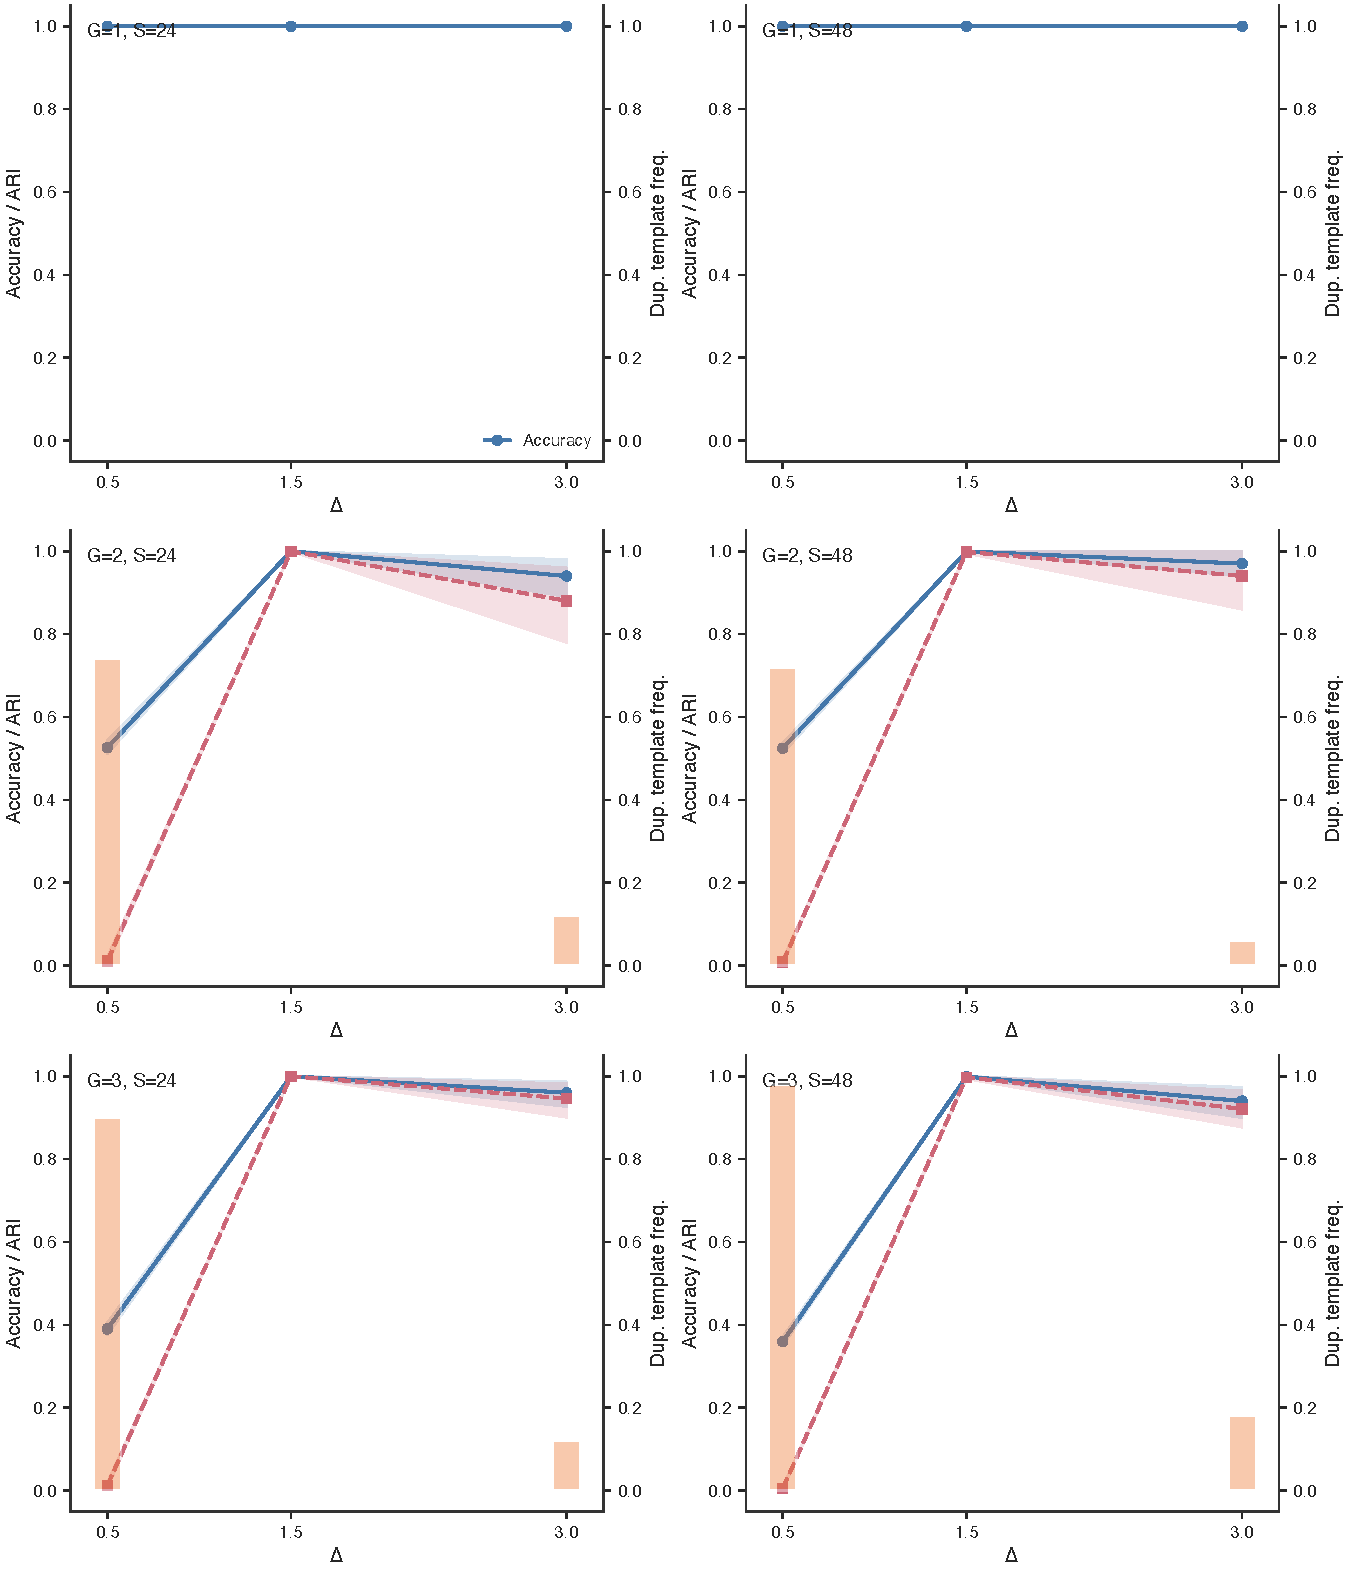
\includegraphics[width=0.96\linewidth]{figures/fig_E05_templates.pdf}
\caption{Finite latent-template score clustering: label-permutation-invariant
hard accuracy (solid) and adjusted Rand index (dashed) vs signal separation $\Delta$,
with 95\% bootstrap bands. Bars show duplicate-template frequency (right axis).
Rows: $G\in\{1,2,3\}$ groups; columns: $S\in\{24,48\}$ sequences per dataset.
At $\Delta=0.5$, group templates collapse for $G\geq2$ and accuracy falls to
near-chance levels. At $\Delta=1.5$, accuracy and ARI approach 1.0.
At $\Delta=3.0$, mean accuracy is $0.940$--$0.970$ for $G=2$ and $0.940$--$0.960$
for $G=3$; duplicate templates appear in $6$--$18$\% of replicates, reflecting
local-optima sensitivity at strong signal.
For $G=1$ ARI is undefined and accuracy is 1.0 by construction.
All 900 objective traces are non-decreasing; no replicate failed.}
\label{fig:planned-templates-paper}
\end{figure}


\begin{table}[!htbp]
\centering
\small
\caption{E05 latent-template score clustering. Accuracy is label-permutation-invariant hard assignment accuracy; ARI is adjusted Rand index (undefined for $G=1$, shown as --). Bootstrap 95\% percentile intervals from 2000 resamples of independently generated datasets. Dup.\ freq.\ is the fraction of replicates where two groups recovered identical templates.}
\label{tab:E05-latent}
\begin{tabular}{@{}lccccccc@{}}
\toprule
$G$ & $S$ & $\Delta$ & $n$ & Accuracy (95\,\% CI) & ARI (95\,\% CI) & Dup.\ freq. & Mon.\ fail \\
\midrule
$1$ & $24$ & $0.5$ & $50$ & $1.000 [1.000,1.000]$ & $--$ & $0.000$ & $0$ \\
$1$ & $24$ & $1.5$ & $50$ & $1.000 [1.000,1.000]$ & $--$ & $0.000$ & $0$ \\
$1$ & $24$ & $3.0$ & $50$ & $1.000 [1.000,1.000]$ & $--$ & $0.000$ & $0$ \\
$1$ & $48$ & $0.5$ & $50$ & $1.000 [1.000,1.000]$ & $--$ & $0.000$ & $0$ \\
$1$ & $48$ & $1.5$ & $50$ & $1.000 [1.000,1.000]$ & $--$ & $0.000$ & $0$ \\
$1$ & $48$ & $3.0$ & $50$ & $1.000 [1.000,1.000]$ & $--$ & $0.000$ & $0$ \\
$2$ & $24$ & $0.5$ & $50$ & $0.526 [0.512,0.542]$ & $0.011 [0.003,0.021]$ & $0.740$ & $0$ \\
$2$ & $24$ & $1.5$ & $50$ & $1.000 [1.000,1.000]$ & $1.000 [1.000,1.000]$ & $0.000$ & $0$ \\
$2$ & $24$ & $3.0$ & $50$ & $0.940 [0.890,0.980]$ & $0.880 [0.780,0.960]$ & $0.120$ & $0$ \\
$2$ & $48$ & $0.5$ & $50$ & $0.525 [0.513,0.537]$ & $0.008 [0.004,0.015]$ & $0.720$ & $0$ \\
$2$ & $48$ & $1.5$ & $50$ & $1.000 [0.999,1.000]$ & $0.998 [0.995,1.000]$ & $0.000$ & $0$ \\
$2$ & $48$ & $3.0$ & $50$ & $0.970 [0.940,1.000]$ & $0.940 [0.860,1.000]$ & $0.060$ & $0$ \\
$3$ & $24$ & $0.5$ & $50$ & $0.390 [0.376,0.405]$ & $0.012 [0.006,0.019]$ & $0.900$ & $0$ \\
$3$ & $24$ & $1.5$ & $50$ & $1.000 [1.000,1.000]$ & $1.000 [1.000,1.000]$ & $0.000$ & $0$ \\
$3$ & $24$ & $3.0$ & $50$ & $0.960 [0.927,0.987]$ & $0.946 [0.901,0.982]$ & $0.120$ & $0$ \\
$3$ & $48$ & $0.5$ & $50$ & $0.360 [0.350,0.371]$ & $0.005 [0.003,0.008]$ & $0.980$ & $0$ \\
$3$ & $48$ & $1.5$ & $50$ & $0.999 [0.998,1.000]$ & $0.997 [0.994,1.000]$ & $0.000$ & $0$ \\
$3$ & $48$ & $3.0$ & $50$ & $0.940 [0.900,0.973]$ & $0.921 [0.877,0.965]$ & $0.180$ & $0$ \\
\bottomrule
\end{tabular}
\end{table}



\FloatBarrier
\subsection{Experiment E06: nonconjugate block-evidence approximations}
The logistic-normal model places a Normal prior $\theta\sim\mathcal{N}(0,4)$ on the
log-odds and integrates out $\theta$ to produce the block log-evidence.
For Bernoulli observations this integral has no closed form; four numerical methods
were evaluated under E06: adaptive mode-centred quadrature (reference),
Laplace, Jaakkola--Jordan (JJ), and expectation propagation (EP).
The label \texttt{pg\_vb} shares the JJ code path and is not an independent method;
it is not benchmarked separately.

\paragraph{Block oracle.}
Block sizes $B\in\{4,8,16,32,64,128\}$, generating probabilities
$p\in\{0.05,0.5,0.95\}$, and 100 independently drawn Bernoulli blocks per cell
(1800 blocks total) were evaluated using the seed scheme
$\mathtt{SeedSequence}([20261021, 6, \textit{cell}, \textit{rep}])$.
The reference is mode-centred adaptive quadrature with $\texttt{epsabs}=10^{-12}$.
Laplace approximation had median absolute log-evidence error $0.021$ and maximum $0.038$.
JJ had median $0.222$ and maximum $0.977$.
JJ is a rigorous variational lower bound on the log-marginal: it produced zero
violations of $\mathrm{JJ}\le\mathrm{reference}+10^{-8}$ across all 1800 blocks.
EP had median absolute error $3.779$ and maximum $30.001$; 1409 of 1800 blocks had
EP above the reference, confirming that parallel EP is not a guaranteed lower bound.
No NaN or infinity was produced by any method on non-degenerate blocks.

The prior-centred Gauss--Hermite quadrature at 200 nodes is inaccurate for large
near-balanced blocks where the posterior is sharply peaked far from the prior centre;
the runner uses mode-centred adaptive quadrature as the reference throughout.

Degenerate blocks (all-success, all-failure at $B\in\{4,8,16,32,64\}$) were tested
separately. EP produced large positive errors on degenerate blocks (e.g., EP error
$11.2$ on $B=64$ all-failure), while Laplace and JJ remained finite and JJ remained
below the reference.

\paragraph{Segmentation propagation.}
One hundred independent Bernoulli sequences were generated with $n=96$,
$k_{\rm true}=3$, boundaries at $(32,64)$, and segment log-odds
$\theta\in\{\mathrm{logit}(0.2),\mathrm{logit}(0.8),\mathrm{logit}(0.2)\}$.
For each sequence, the full dynamic program was run with each method's approximate
block-evidence table, and results were compared to the quadrature reference.
Laplace caused 1 of 100 MAP mismatches versus reference; JJ caused 19; EP caused 89.
Mean maximum absolute difference in $p(k|y)$ was $0.013$ for Laplace, $0.056$ for JJ,
and $0.236$ for EP. Mean $\mathrm{F}_1@3$ was $0.530$ for Laplace, $0.545$ for JJ,
and $0.423$ for EP, versus $0.503$ for the quadrature reference.
EP's large block-score errors propagated into substantially wrong posteriors in most
sequences.

\paragraph{Error bound status.}
JJ is a variational lower bound on the block log-evidence, not an upper bound on the
approximation error. Theorem~\ref{thm:stability-paper} provides bounds on the partition
posterior conditional on a uniform block-score error over all admissible segments. The
theorem's conditional conclusion holds but does not certify any specific method's errors
without externally verifying that the method's errors are uniformly bounded. For E06, only
the reference quadrature and the Laplace approximation have bounded errors on all tested
cells; EP errors are not uniformly bounded.

\begin{figure}[ht]
\centering
\begin{subfigure}[t]{0.98\textwidth}
  \centering
  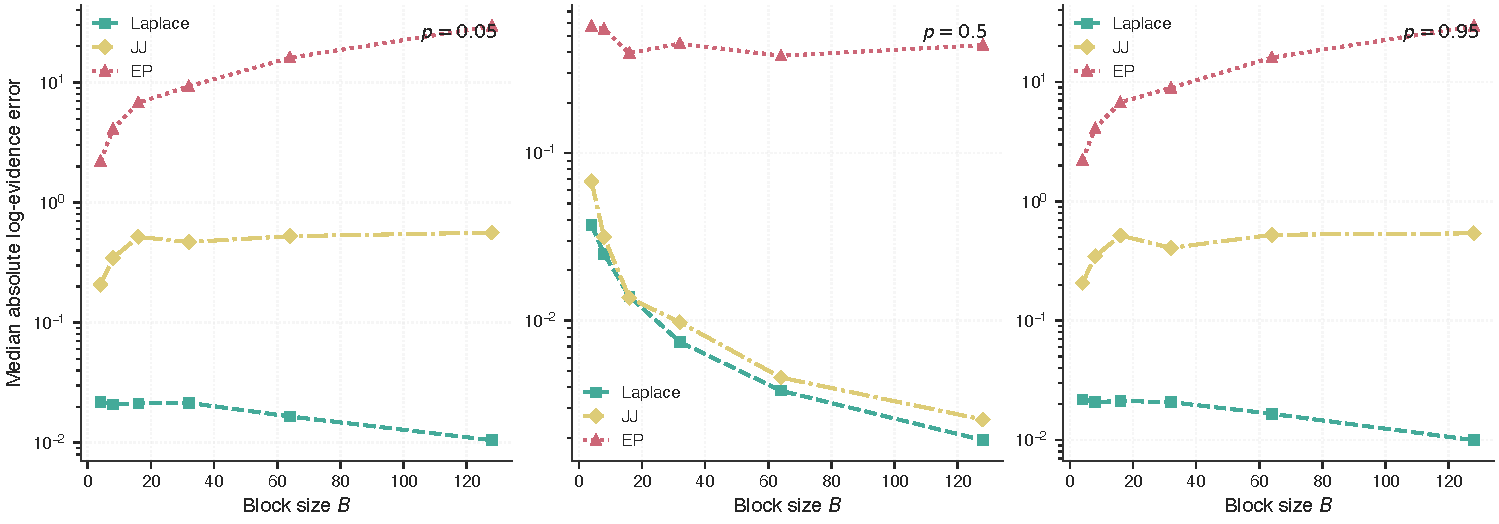
\includegraphics[width=\textwidth]{figures/fig_E06_local_error}
  \caption{Median absolute log-evidence error by block size $B$ and generating success probability
  $p$. Laplace errors are small (median $|\Delta\log Z|=0.021$, max $0.038$) and decrease
  with $B$ at balanced $p$. JJ errors are uniformly negative (lower bound) with median
  $0.22$ and maximum $0.98$; errors are larger at extreme $p$ values. EP errors are large
  (median $3.78$, max $30.0$) and systematically positive for extreme $p$, reflecting
  that parallel EP is not a guaranteed lower bound on the log-marginal.}
  \label{fig:e06-local-error}
\end{subfigure}

\vspace{1em}

\begin{subfigure}[t]{0.98\textwidth}
  \centering
  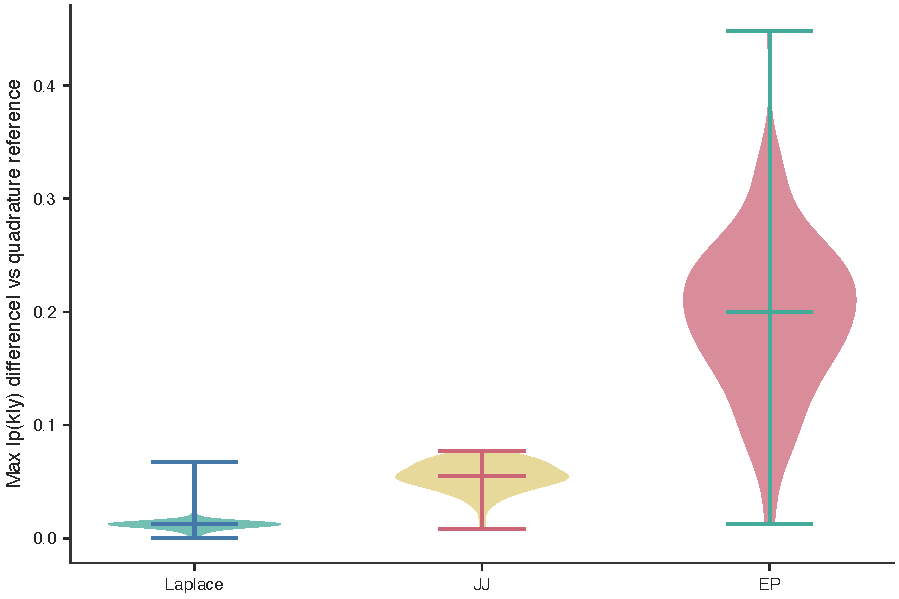
\includegraphics[width=\textwidth]{figures/fig_E06_global_error}
  \caption{Segmentation propagation discrepancies versus the quadrature reference
  ($n=96$, $k_{\rm true}=3$, boundaries at $(32,64)$, 100 independent sequences).
  Laplace: mean max $|p(k|y)|$ difference $0.013$, 1 MAP mismatch. JJ: mean $0.056$,
  19 MAP mismatches. EP: mean $0.236$, 89 MAP mismatches.
  EP boundary-marginal discrepancies reach $0.84$ in individual sequences.}
  \label{fig:e06-global-error}
\end{subfigure}

\caption{Experiment E06: local and global effects of nonconjugate block-evidence
approximations. (a) Absolute log-evidence error by block size and success probability.
(b) Count posterior and boundary-marginal discrepancies in the segmentation propagation
experiment. Reference in both panels is mode-centred adaptive quadrature
($\texttt{epsabs}=10^{-12}$).}
\label{fig:planned-nonconjugate-paper}
\end{figure}


\begin{table}[ht]
\centering
\caption{Nonconjugate block-evidence approximations for the
Bernoulli logistic-normal model. Block sizes $B\in\{4,8,16,32,64,128\}$,
generating probabilities $p\in\{0.05,0.5,0.95\}$, 100 independent replicates per cell
(1800 blocks total). Prior $\theta\sim\mathcal{N}(0,4)$. Reference: mode-centred
adaptive quadrature ($\texttt{epsabs}=10^{-12}$). \texttt{pg\_vb} is an alias of JJ
in the estimator and is not listed separately. JJ LB column: count of blocks where
JJ exceeds reference by more than $10^{-8}$ (0 of 1800: JJ is a verified lower bound).
EP is \emph{not} a guaranteed lower bound; 1409 of 1800 blocks have EP above the
reference. Runtimes are per-block medians on a single CPU core.}
\label{tab:planned-nonconjugate-paper}
\begin{tabular}{lrrrr}
\toprule
Method & Median $|\Delta\log Z|$ & Max $|\Delta\log Z|$ & JJ LB violations & Median runtime \\
\midrule
Laplace        & $0.021$ & $0.038$ & N/A        & $0.050$\,ms \\
JJ (pg\_vb alias) & $0.222$ & $0.977$ & $0/1800$ & $0.235$\,ms \\
EP             & $3.779$ & $30.001$ & N/A (not LB) & $2.093$\,ms \\
\bottomrule
\end{tabular}
\end{table}


\FloatBarrier
\subsection{Experiment E07: misspecification and missing data}
The robustness of boundary recovery to distributional misspecification and missing
observations was evaluated under E07.
Data were generated at $n=256$, $k_{\rm true}=3$, true boundaries $(85,170)$,
with segment means $(0,1.5,0)$ and independent noise.
Four data-generating classes were used: (a) Gaussian reference with $N(0,1)$ noise
fit by a known-variance Gaussian model (correct specification);
(b) Student $t_3/\sqrt{3}$ noise fit by the Gaussian model (misspecified, heavy tail);
(c) Negative-Binomial counts with dispersion $r=2$ and means $(2,5,2)$ fit by both
Poisson (misspecified) and NegBin at fixed $r=2$ (correct);
(d) Beta-Binomial counts with $m=20$ and intra-class correlation $0.1$ at success
probabilities $(0.2,0.6,0.2)$ fit by Binomial (misspecified, overdispersed).
Four missingness conditions were crossed with each family: no missingness, MCAR 10\%,
MCAR 30\%, and a single contiguous missing block of $\lfloor 0.15n\rfloor = 38$
observations drawn uniformly from the interior.
Each applicable combination used 100 independent datasets under the
seed scheme $\mathtt{SeedSequence}([20261021,7,\textit{cell},\textit{rep}])$.
Prior: geometric-decay count, $\mathcal{N}(0,4)$ Gaussian segment prior,
$\mathrm{Gamma}(2,1)$ Poisson prior, $\mathrm{Beta}(2,3)$ NegBin/Binomial prior;
$k_{\max}=10$.

\paragraph{Correct specification.}
Under correct Gaussian specification and no missingness, mean
$\mathrm{F}_1@3$ was $0.918$ $[0.881, 0.950]$ and count exact-match was
$0.960$. MCAR 30\% reduced $\mathrm{F}_1@3$ to $0.809$ $[0.760, 0.856]$;
the contiguous missing block (38 of 256 observations) further reduced
$\mathrm{F}_1@3$ to $0.721$ $[0.659, 0.783]$, while count exact-match
remained at $0.970$ for both conditions.
The correctly specified NegBin fit on NegBin data achieved $\mathrm{F}_1@3$
of $0.709$ $[0.636, 0.774]$ under no missingness, with count exact-match
$0.970$.

\paragraph{Heavy-tail misspecification.}
Fitting a Gaussian model to Student $t_3/\sqrt{3}$ data produced mean
$\mathrm{F}_1@3$ of $0.767$ $[0.721, 0.814]$ under no missingness, compared
to $0.918$ for the correct Gaussian specification.
Count exact-match fell to $0.530$, indicating that heavy-tailed noise
shifted the count posterior toward $k>3$.
MCAR 10\% improved $\mathrm{F}_1@3$ slightly to $0.804$,
reflecting the reduced influence of outlying observations under light missingness.

\paragraph{Overdispersion misspecification.}
Fitting a Poisson model to NegBin-generated data achieved $\mathrm{F}_1@3$
of $0.525$ $[0.472, 0.580]$ under no missingness, versus $0.709$ for the
correctly specified NegBin fit: a difference of $0.184$ in favor of the
correctly specified model.
Count exact-match was $0.290$ for the Poisson fit versus $0.970$ for NegBin,
with the Poisson model absorbing overdispersion as additional changepoints.
Fitting a Binomial model to Beta-Binomial data produced the largest
degradation: $\mathrm{F}_1@3$ of $0.464$ $[0.431, 0.500]$ and count
exact-match of only $0.060$ under no missingness (most replicates selected
$k>3$). The contiguous missing block further reduced $\mathrm{F}_1@3$ to
$0.365$ $[0.327, 0.406]$.

\paragraph{Numerical behavior.}
No NaN or non-finite log-evidence was observed in any of the 2000 replicates.
The gate threshold (failure rate below 5\%) was satisfied for all 20 cells.

\begin{figure}[!htbp]
\centering
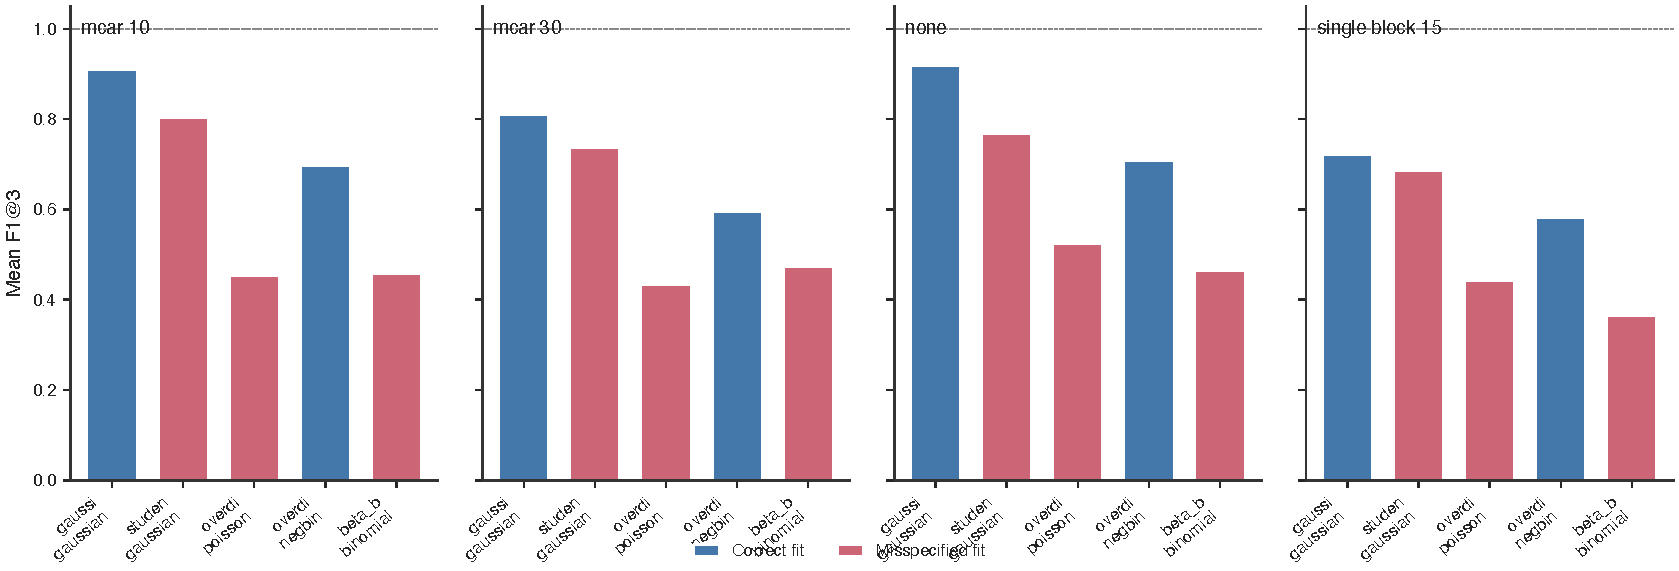
\includegraphics[width=0.98\linewidth]{figures/fig_E07_robustness.pdf}
\caption{E07 misspecification and missing data: mean MAP boundary $\mathrm{F}_1@3$
by data-generating family (rows within each panel) and missingness condition (columns).
Blue bars: correctly specified fits; coral bars: misspecified fits.
Gaussian reference with correct Gaussian fit (blue) provides the baseline.
Student $t_3$ data fit by Gaussian (coral) shows moderate degradation.
NegBin data fit by Poisson (coral) shows larger degradation; the correct NegBin fit
(blue) recovers substantially higher accuracy.
Beta-Binomial data fit by Binomial (coral) shows the largest degradation:
overdispersion inflates the apparent segment count.
All 2000 replicates (20 cells $\times$ 100 each) completed with no numerical failures.
}
\label{fig:E07-robustness-paper}
\end{figure}


\begin{table}[!htbp]
\centering
\footnotesize
\caption{Boundary recovery under misspecification and missing data. $\mathrm{F_1}@3$ is mean $[95\%\ \mathrm{CI}]$ across 100 independent replicates. $\dag$ denotes a misspecified fit. MCAR: missing completely at random; Block: a single contiguous missing region of $\lfloor 0.15n \rfloor$ observations.}
\label{tab:E07-robustness}
\begin{tabular}{llccccc}
\toprule
Generating data & Fitted model & Missingness & $\mathrm{F_1}@3$ [95\% CI] & Count exact & $p(k^\star\!\mid y)$ & Brier$_k$ \\
\midrule
Gaussian & Gaussian & None         & 0.918 [0.881,\,0.950] & 0.960 & 0.764 & 0.1221 \\
Gaussian & Gaussian & MCAR 10\%   & 0.909 [0.870,\,0.946] & 0.970 & 0.749 & 0.1268 \\
Gaussian & Gaussian & MCAR 30\%   & 0.809 [0.760,\,0.856] & 0.970 & 0.752 & 0.1259 \\
Gaussian & Gaussian & Block 15\%  & 0.721 [0.659,\,0.783] & 0.970 & 0.741 & 0.1342 \\
Student $t_3$ & Gaussian$^\dag$ & None        & 0.767 [0.721,\,0.814] & 0.530 & 0.434 & 0.6780 \\
Student $t_3$ & Gaussian$^\dag$ & MCAR 10\%  & 0.804 [0.758,\,0.848] & 0.610 & 0.499 & 0.5789 \\
Student $t_3$ & Gaussian$^\dag$ & MCAR 30\%  & 0.737 [0.684,\,0.788] & 0.610 & 0.480 & 0.5758 \\
Student $t_3$ & Gaussian$^\dag$ & Block 15\% & 0.685 [0.629,\,0.744] & 0.670 & 0.520 & 0.5208 \\
Neg.\ Binomial & Poisson$^\dag$ & None        & 0.525 [0.472,\,0.580] & 0.290 & 0.178 & 0.8937 \\
Neg.\ Binomial & Poisson$^\dag$ & MCAR 10\%  & 0.454 [0.401,\,0.506] & 0.320 & 0.202 & 0.8537 \\
Neg.\ Binomial & Poisson$^\dag$ & MCAR 30\%  & 0.433 [0.373,\,0.495] & 0.360 & 0.210 & 0.8318 \\
Neg.\ Binomial & Poisson$^\dag$ & Block 15\% & 0.443 [0.380,\,0.505] & 0.360 & 0.205 & 0.8546 \\
Neg.\ Binomial & Neg.\ Binomial & None        & 0.709 [0.636,\,0.774] & 0.970 & 0.678 & 0.1845 \\
Neg.\ Binomial & Neg.\ Binomial & MCAR 10\%  & 0.698 [0.638,\,0.758] & 0.980 & 0.685 & 0.1712 \\
Neg.\ Binomial & Neg.\ Binomial & MCAR 30\%  & 0.595 [0.525,\,0.660] & 0.980 & 0.640 & 0.2143 \\
Neg.\ Binomial & Neg.\ Binomial & Block 15\% & 0.582 [0.518,\,0.645] & 0.950 & 0.644 & 0.2139 \\
Beta-Binomial & Binomial$^\dag$ & None        & 0.464 [0.431,\,0.500] & 0.060 & 0.043 & 1.2514 \\
Beta-Binomial & Binomial$^\dag$ & MCAR 10\%  & 0.458 [0.428,\,0.492] & 0.040 & 0.025 & 1.2918 \\
Beta-Binomial & Binomial$^\dag$ & MCAR 30\%  & 0.474 [0.431,\,0.522] & 0.120 & 0.065 & 1.1790 \\
Beta-Binomial & Binomial$^\dag$ & Block 15\% & 0.365 [0.327,\,0.406] & 0.070 & 0.039 & 1.2577 \\
\bottomrule
\end{tabular}
\end{table}



\FloatBarrier
\subsection{Experiment E10: computational scaling}
\label{sec:e10}
Experiment E10 measured wall-clock time and peak memory for $n\in\{128,256,512,1024,2048\}$ and $k_{\max}\in\{5,10,20\}$ (15 cells, 0 failures) on a Gaussian sequence with $k_{\rm true}=3$ fixed boundaries. Each cell was timed over 7 repeats after a warmup pass with BLAS pinned to 1 thread. Table~\ref{tab:E10-scaling-paper} reports median timings; Figure~\ref{fig:E10-scaling-paper} shows log-log scaling.

Peak memory at $n=2048$ was $500.7$ MB across all $k_{\max}$ values, consistent with $O(n^2)$ storage of the block-evidence matrix; the log-log slope in $n$ from $n=128$ to $n=2048$ at $k_{\max}=20$ was $1.94$--$2.00$ (converging). Forward-backward runtime had log-log slope $1.10$--$1.24$ in $n$ at $k_{\max}=20$; end-to-end runtime at $n=2048$, $k_{\max}=20$ was $3.25$ seconds ($3.02$ seconds forward-backward, $0.10$ seconds block evidence). These slopes summarize this implementation over the measured finite range; they do not replace the $\Theta(k_{\max}n^2)$ worst-case bound in Proposition~\ref{prop:complexity-paper}.

\begin{figure}[!htbp]
\centering
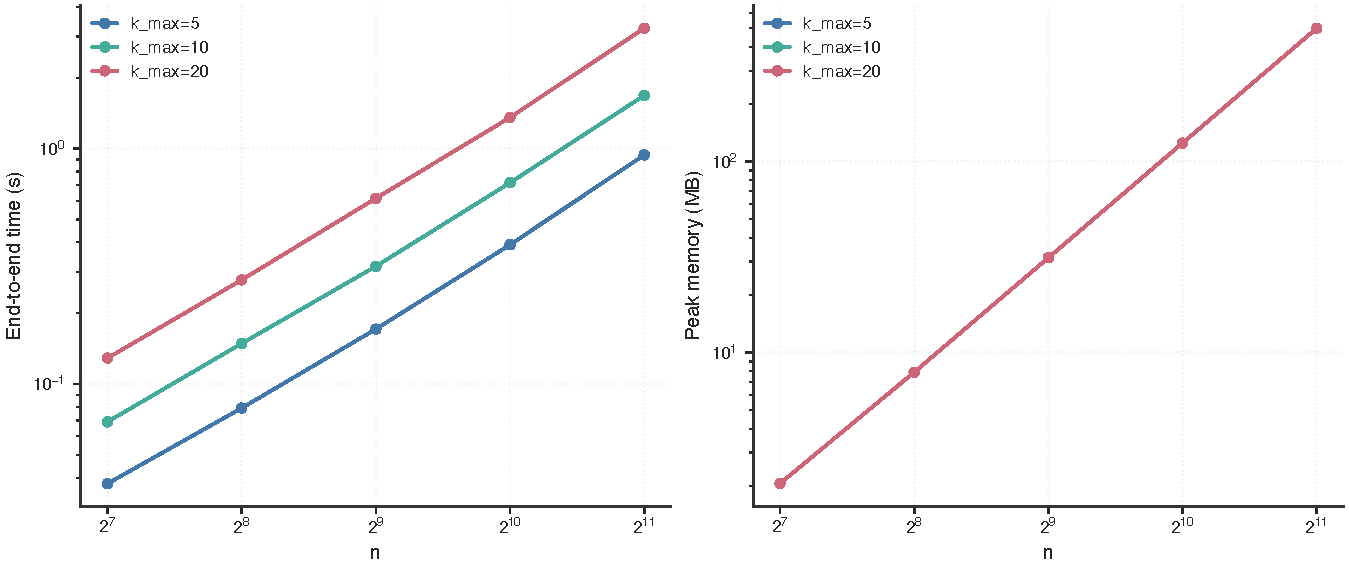
\includegraphics[width=0.98\linewidth]{figures/fig_E10_scaling.pdf}
\caption{Computational scaling. Left: end-to-end wall-clock time (log scale) versus
sequence length $n$ at $k_{\max}\in\{5,10,20\}$; right: peak memory (MB, log scale) versus $n$.
Dashed lines are $O(n^2)$ and $O(n^{1.14})$ references. Timings are medians over 7 repeats per cell;
BLAS pinned to 1 thread. Config SHA256: \texttt{bece422c9d90093f}.}
\label{fig:E10-scaling-paper}
\end{figure}


\begin{table}[!htbp]
\centering
\caption{Computational scaling benchmark: median wall-clock time (seconds) and peak memory (MB)
over 7 timed repeats per cell. Block evidence and forward-backward timings are from direct
DP function calls; end-to-end includes all setup and post-processing. BLAS threads pinned
to 1. Gaussian family, $\nu=0$, $\rho^2=4$, $\sigma^2=1$; geometric-decay count prior;
Apple Silicon, Python 3.11, NumPy 2.4.6. Config SHA256: \texttt{bece422c9d90093f}.}
\label{tab:E10-scaling-paper}
\small
\begin{tabular}{rrrrrrr}
\toprule
$n$ & $k_{\max}$ & $k_{\rm map}$ & Block (s) & Fwd-bwd (s) & E2E (s) & Mem (MB)\\
\midrule
128 & 5 & 3 & 0.0004 & 0.0328 & 0.0377 & 2.1\\
128 & 10 & 3 & 0.0004 & 0.0639 & 0.0691 & 2.1\\
128 & 20 & 3 & 0.0004 & 0.1252 & 0.1289 & 2.1\\
256 & 5 & 3 & 0.0012 & 0.0690 & 0.0790 & 7.9\\
256 & 10 & 3 & 0.0013 & 0.1378 & 0.1487 & 7.9\\
256 & 20 & 3 & 0.0014 & 0.2690 & 0.2769 & 7.9\\
512 & 5 & 3 & 0.0057 & 0.1460 & 0.1711 & 31.4\\
512 & 10 & 3 & 0.0060 & 0.2906 & 0.3163 & 31.4\\
512 & 20 & 3 & 0.0058 & 0.5791 & 0.6151 & 31.4\\
1024 & 5 & 3 & 0.0207 & 0.3202 & 0.3905 & 125.3\\
1024 & 10 & 3 & 0.0224 & 0.6428 & 0.7164 & 125.3\\
1024 & 20 & 3 & 0.0210 & 1.2776 & 1.3572 & 125.3\\
2048 & 5 & 3 & 0.0954 & 0.7473 & 0.9403 & 500.7\\
2048 & 10 & 3 & 0.0918 & 1.4748 & 1.6827 & 500.7\\
2048 & 20 & 3 & 0.1025 & 3.0226 & 3.2483 & 500.7\\
\bottomrule
\end{tabular}

\end{table}


\FloatBarrier
\subsection{Experiment E09: real-data analysis}
\label{sec:e09}
Table~\ref{tab:real-summary-paper} summarizes the E09 real-data fits (canonical artifact \texttt{0f5281c46ee8976e}, protocol revision 2026-10-24-2). Each fit used the geometric-decay-log4 count prior and the data sources identified by their SHA256 checksums in the artifact. The DP invariants were verified for all resolved fits. The fitted segmentations establish descriptive posterior behavior; these datasets do not include independently verified external boundary annotations, so boundary recovery accuracy against ground truth cannot be reported.

\textit{Truncation criterion.} A fit is truncated when $\hat k = k_{\max}$ or $P(k = k_{\max} \mid y) \geq 0.01$. A truncated fit has unknown unrestricted MAP segment count; it does not establish the number of segments under an untruncated prior.

\begin{table}[!htbp]
\centering
\small
\caption{Real-data segmentations (artifact \texttt{0f5281c46ee8976e}). Prior: geometric-decay log4 for resolved fits; uniform prior also shown where resolved. Log evidences arise from different data models and are not directly comparable across rows. $\dagger$ Truncated: $P(k=k_{\max}\mid y) > 0$; unrestricted MAP unknown. Eight curated rows (one per dataset--prior combination); full 31-cell protocol recorded in the artifact.}
\label{tab:real-summary-paper}
\begin{tabularx}{\columnwidth}{@{}Y C{0.19\columnwidth} C{0.12\columnwidth} C{0.28\columnwidth}@{}}
\toprule
Case & $n$ or shape & $\widehat k$ & Log evidence \\
\midrule
Well-log full (geometric) & 4050 & 83 & $-37906.09$ \\
Well-log full (uniform) & 4050 & $100^{\dagger}$ & $-37784.74$ \\
Well-log stride-8 (geometric) & 507 & 25 & $-4901.80$ \\
Well-log stride-8 (uniform) & 507 & 37 & $-4864.93$ \\
CGH single subject (geometric) & 2215 & 71 & $1700.43$ \\
CGH pooled 43 subjects (geometric) & $2215\times43$ & $60^{\dagger}$ & $41222.49$ \\
Methylation (geometric) & 1904 & $120^{\dagger}$ & $1453.78$ \\
Methylation (uniform) & 1904 & $120^{\dagger}$ & $1614.25$ \\
\bottomrule
\end{tabularx}
\end{table}


\paragraph{Well-log.}
The full well-log sequence contains 4,050 NMR values. Under the geometric-decay-log4 prior with $k_{\max}=100$, the Gaussian fit selected $k_{\max}=83$ segments with $k_{\max}=82$ internal changepoints (log evidence $-37906.09$, $P(k=83 \mid y) = 1 - 3.2 \times 10^{-6}$; resolved) (Figure~\ref{fig:welllog-paper}). Under the uniform count prior with the same $k_{\max}=100$, the fit selected $100$ segments and was truncated ($P(k=100 \mid y) = 0.344$); the unrestricted MAP under the uniform prior is unknown.

Minimum-segment-length sensitivity: requiring $\min\_seg \geq 5$ gave $k_{\max}=61$ (resolved); $\min\_seg \geq 10$ gave $k_{\max}=56$ (resolved). These fits use a different constrained partition prior whose normalizer $C_k$ differs from the unconstrained case; their log evidences are not directly comparable as Bayes factors against the $\min\_seg=1$ fit.

For the stride-8 subsample ($n=507$, every eighth observation), the geometric prior gave $k_{\max}=25$ (resolved at $k_{\max}=60$, log evidence $-4901.80$) and the uniform prior gave $k_{\max}=37$ (resolved, log evidence $-4864.93$). The two segment counts do not represent a quantifiable fraction of the full-sequence structure because the same prior over partitions is not applied to both sequences.

A supplemental comparison with ruptures v1.1.10 PELT under a BIC penalty ($2 \hat{\sigma}^2_{\rm MAD} \log n$) gave 58 segments on the full sequence versus BayesBreak's 83 (geometric prior). Boundary-set agreement $F_1@3$ between PELT and BayesBreak was $0.0$ at this scale. PELT and BayesBreak optimize different objectives under different model assumptions; their boundary sets are not compared against an external reference.

\begin{figure}[!htbp]
  \centering
  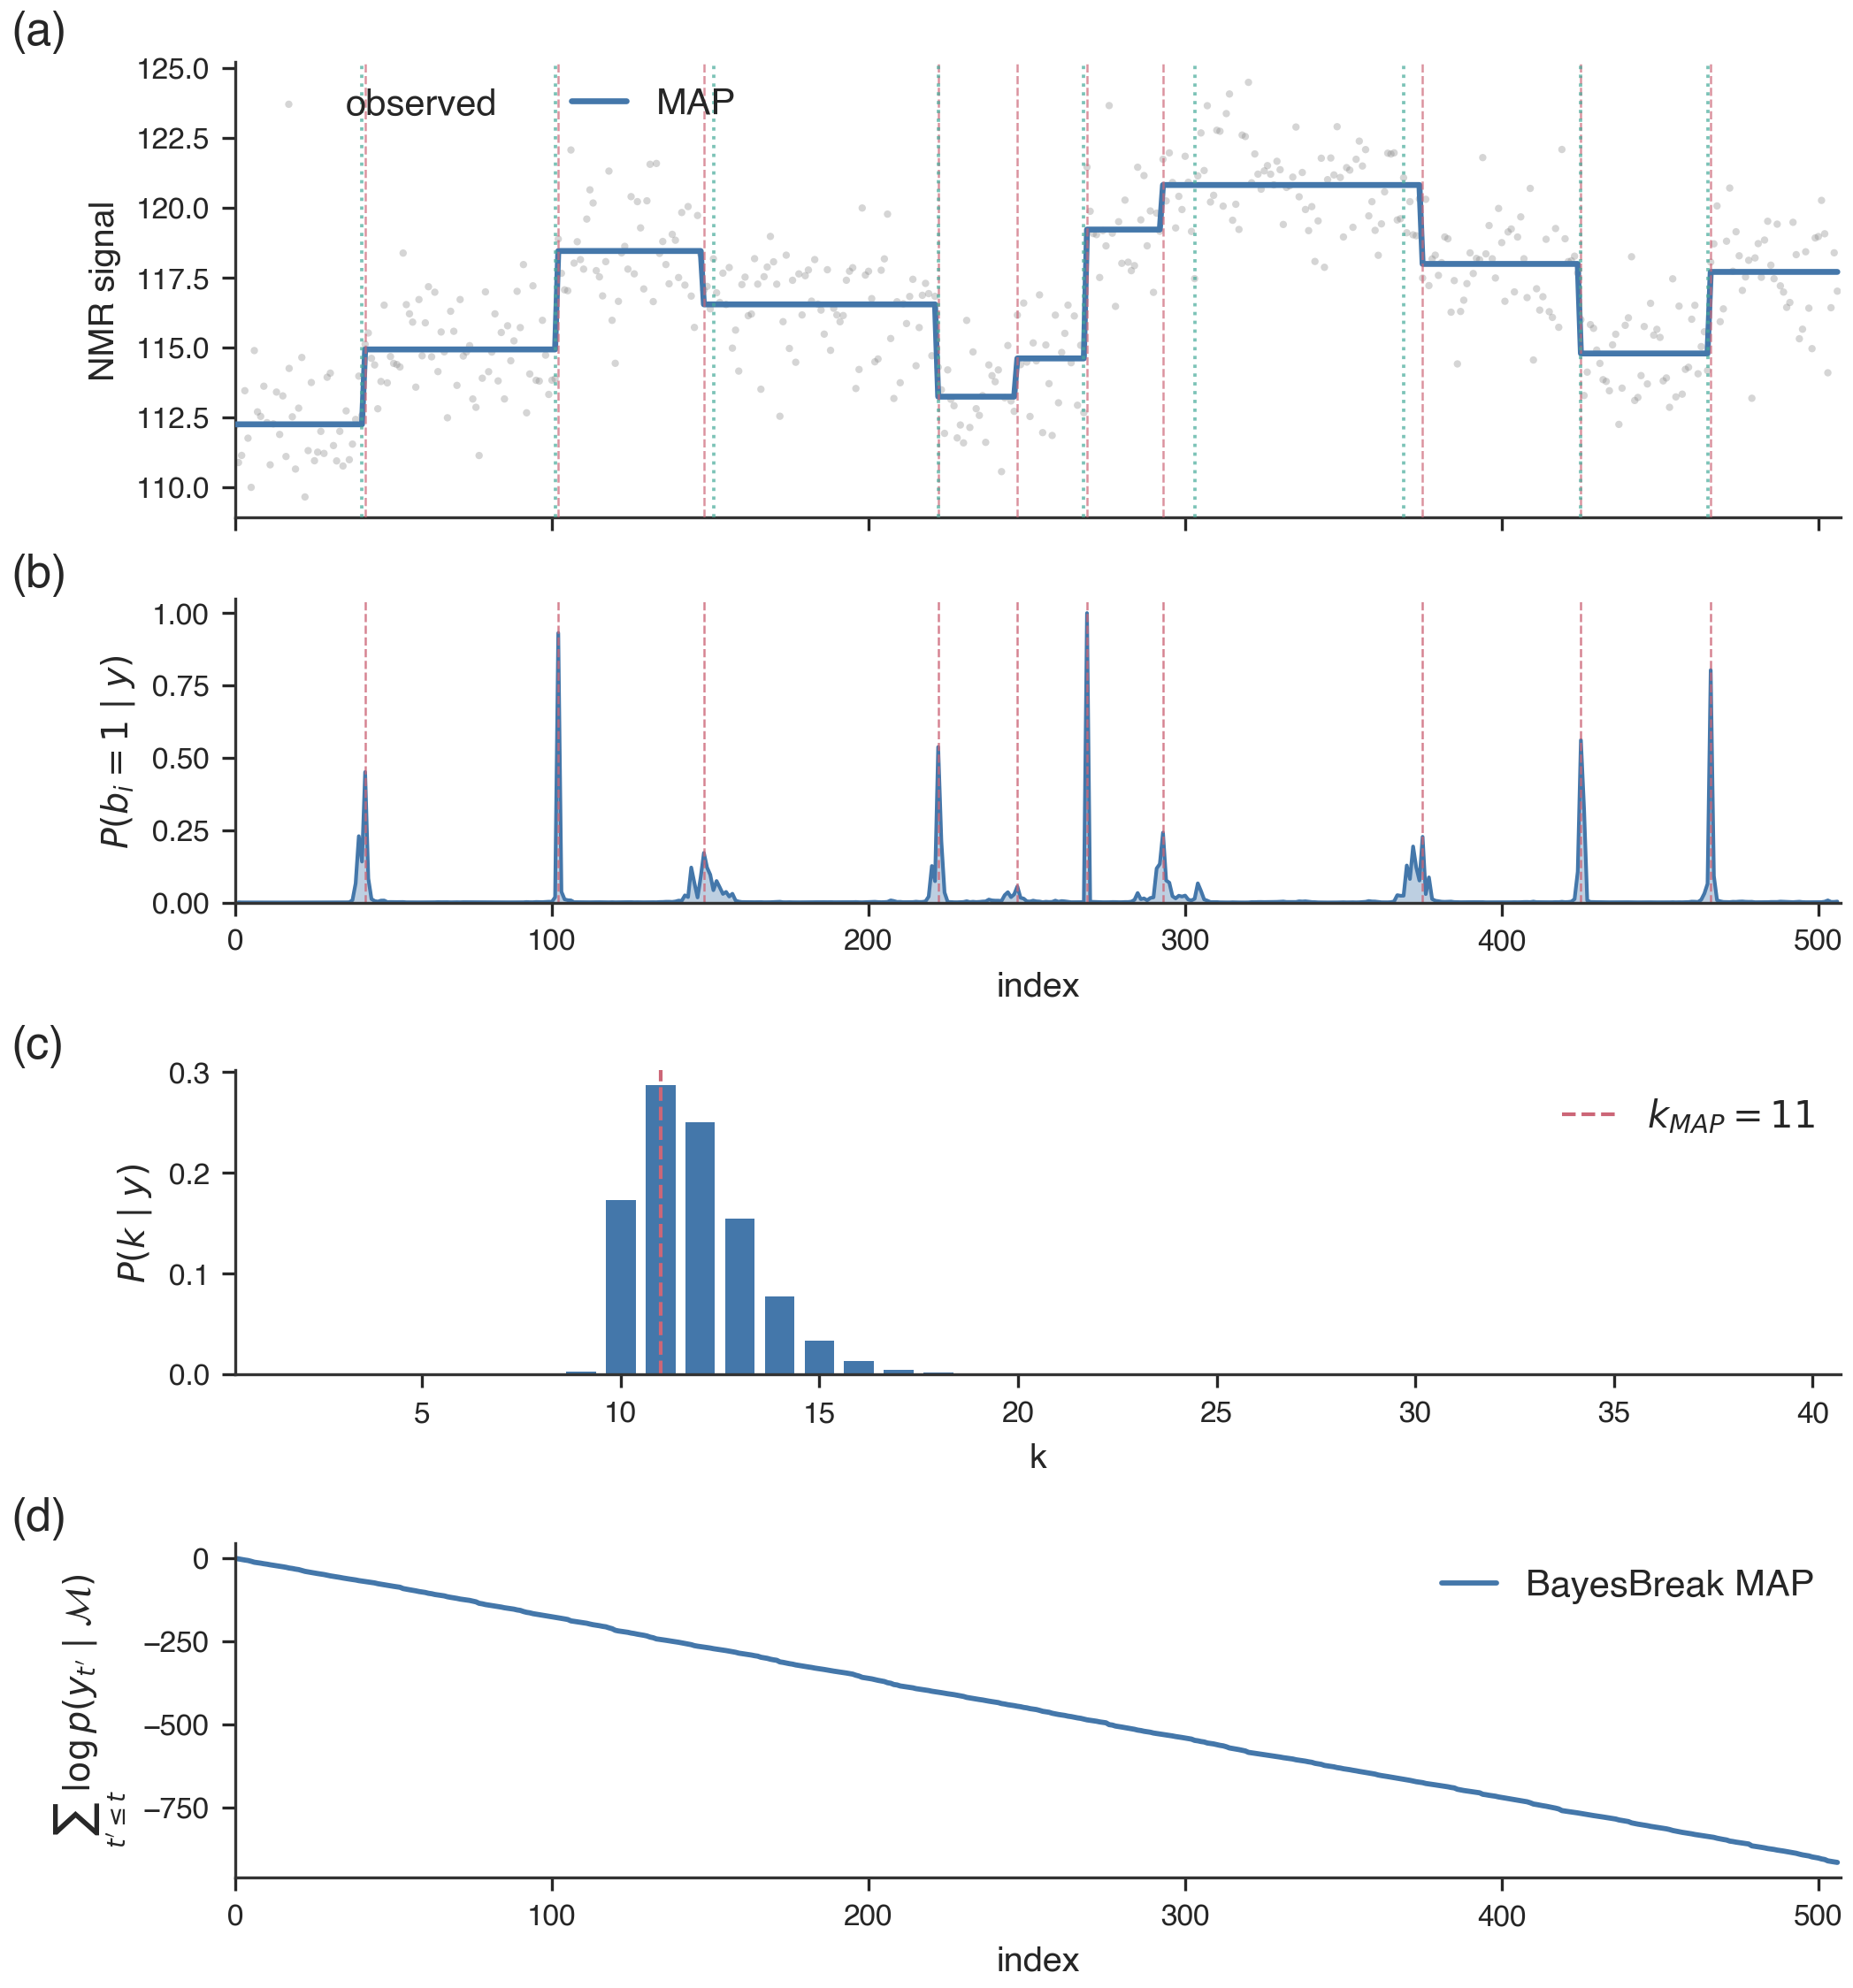
\includegraphics[width=0.90\textwidth,height=0.43\textheight,keepaspectratio]{paper/figures/fig6_welllog.png}
  \caption{Well-log segmentation. Solid segmentation and red markers are fitted summaries;
    boundary probabilities and $p(k\mid y)$ are posterior quantities;
    the cumulative panel is in-sample.}
  \label{fig:welllog-paper}
\end{figure}


\paragraph{Array-CGH.}
The data are the \texttt{ecp} package \texttt{ACGH.RData} matrix ($2{,}215$ probes, 43 subjects). Subject 0 was analyzed independently using the per-probe per-subject sample-weight array (\texttt{sample\_weight} shape $2215 \times 43$; subject-0 column passed as \texttt{sample\_weight}). Under the geometric prior with $k_{\max}=100$, subject 0 returned $k_{\max}=71$ (71 segments, 70 internal changepoints; resolved, log evidence $1700.43$, $P(k=71 \mid y) = 1 - 3.8 \times 10^{-16}$) (Figure~\ref{fig:cgh-paper}).

The pooled shared-boundary analysis used \texttt{SharedBoundaryReplicatesSegmenter} on all 43 subjects simultaneously. The pooled fit was truncated at every tested $k_{\max}$ up to 60 ($P(k=60 \mid y) = 1.0$ at $k_{\max}=60$). The unrestricted pooled MAP segment count is unknown; $k > 60$ is certain. The summed per-subject log evidences under an independent-fits model and the pooled log evidence arise from different partition priors and are not a Bayes factor between the pooled and independent models.

Exact boundary-event marginals $P(b_i = 1 \mid y, k_{\max}=71)$ were computed from the fitted DP for subject 0 (supplemental artifact \texttt{dc8432589c3fa528}). The invariant $\sum_i P(b_i = 1 \mid y, k_{\max}=71) = k_{\max} - 1 = 70$ was verified. These marginals quantify boundary uncertainty conditional on $k_{\max}=71$; they are not marginalised over the count posterior.

No chromosome-coordinate or arm-level genomic annotation was performed. The reported boundaries are probe-index positions, not genomic coordinates.

\begin{figure}[!htbp]
  \centering
  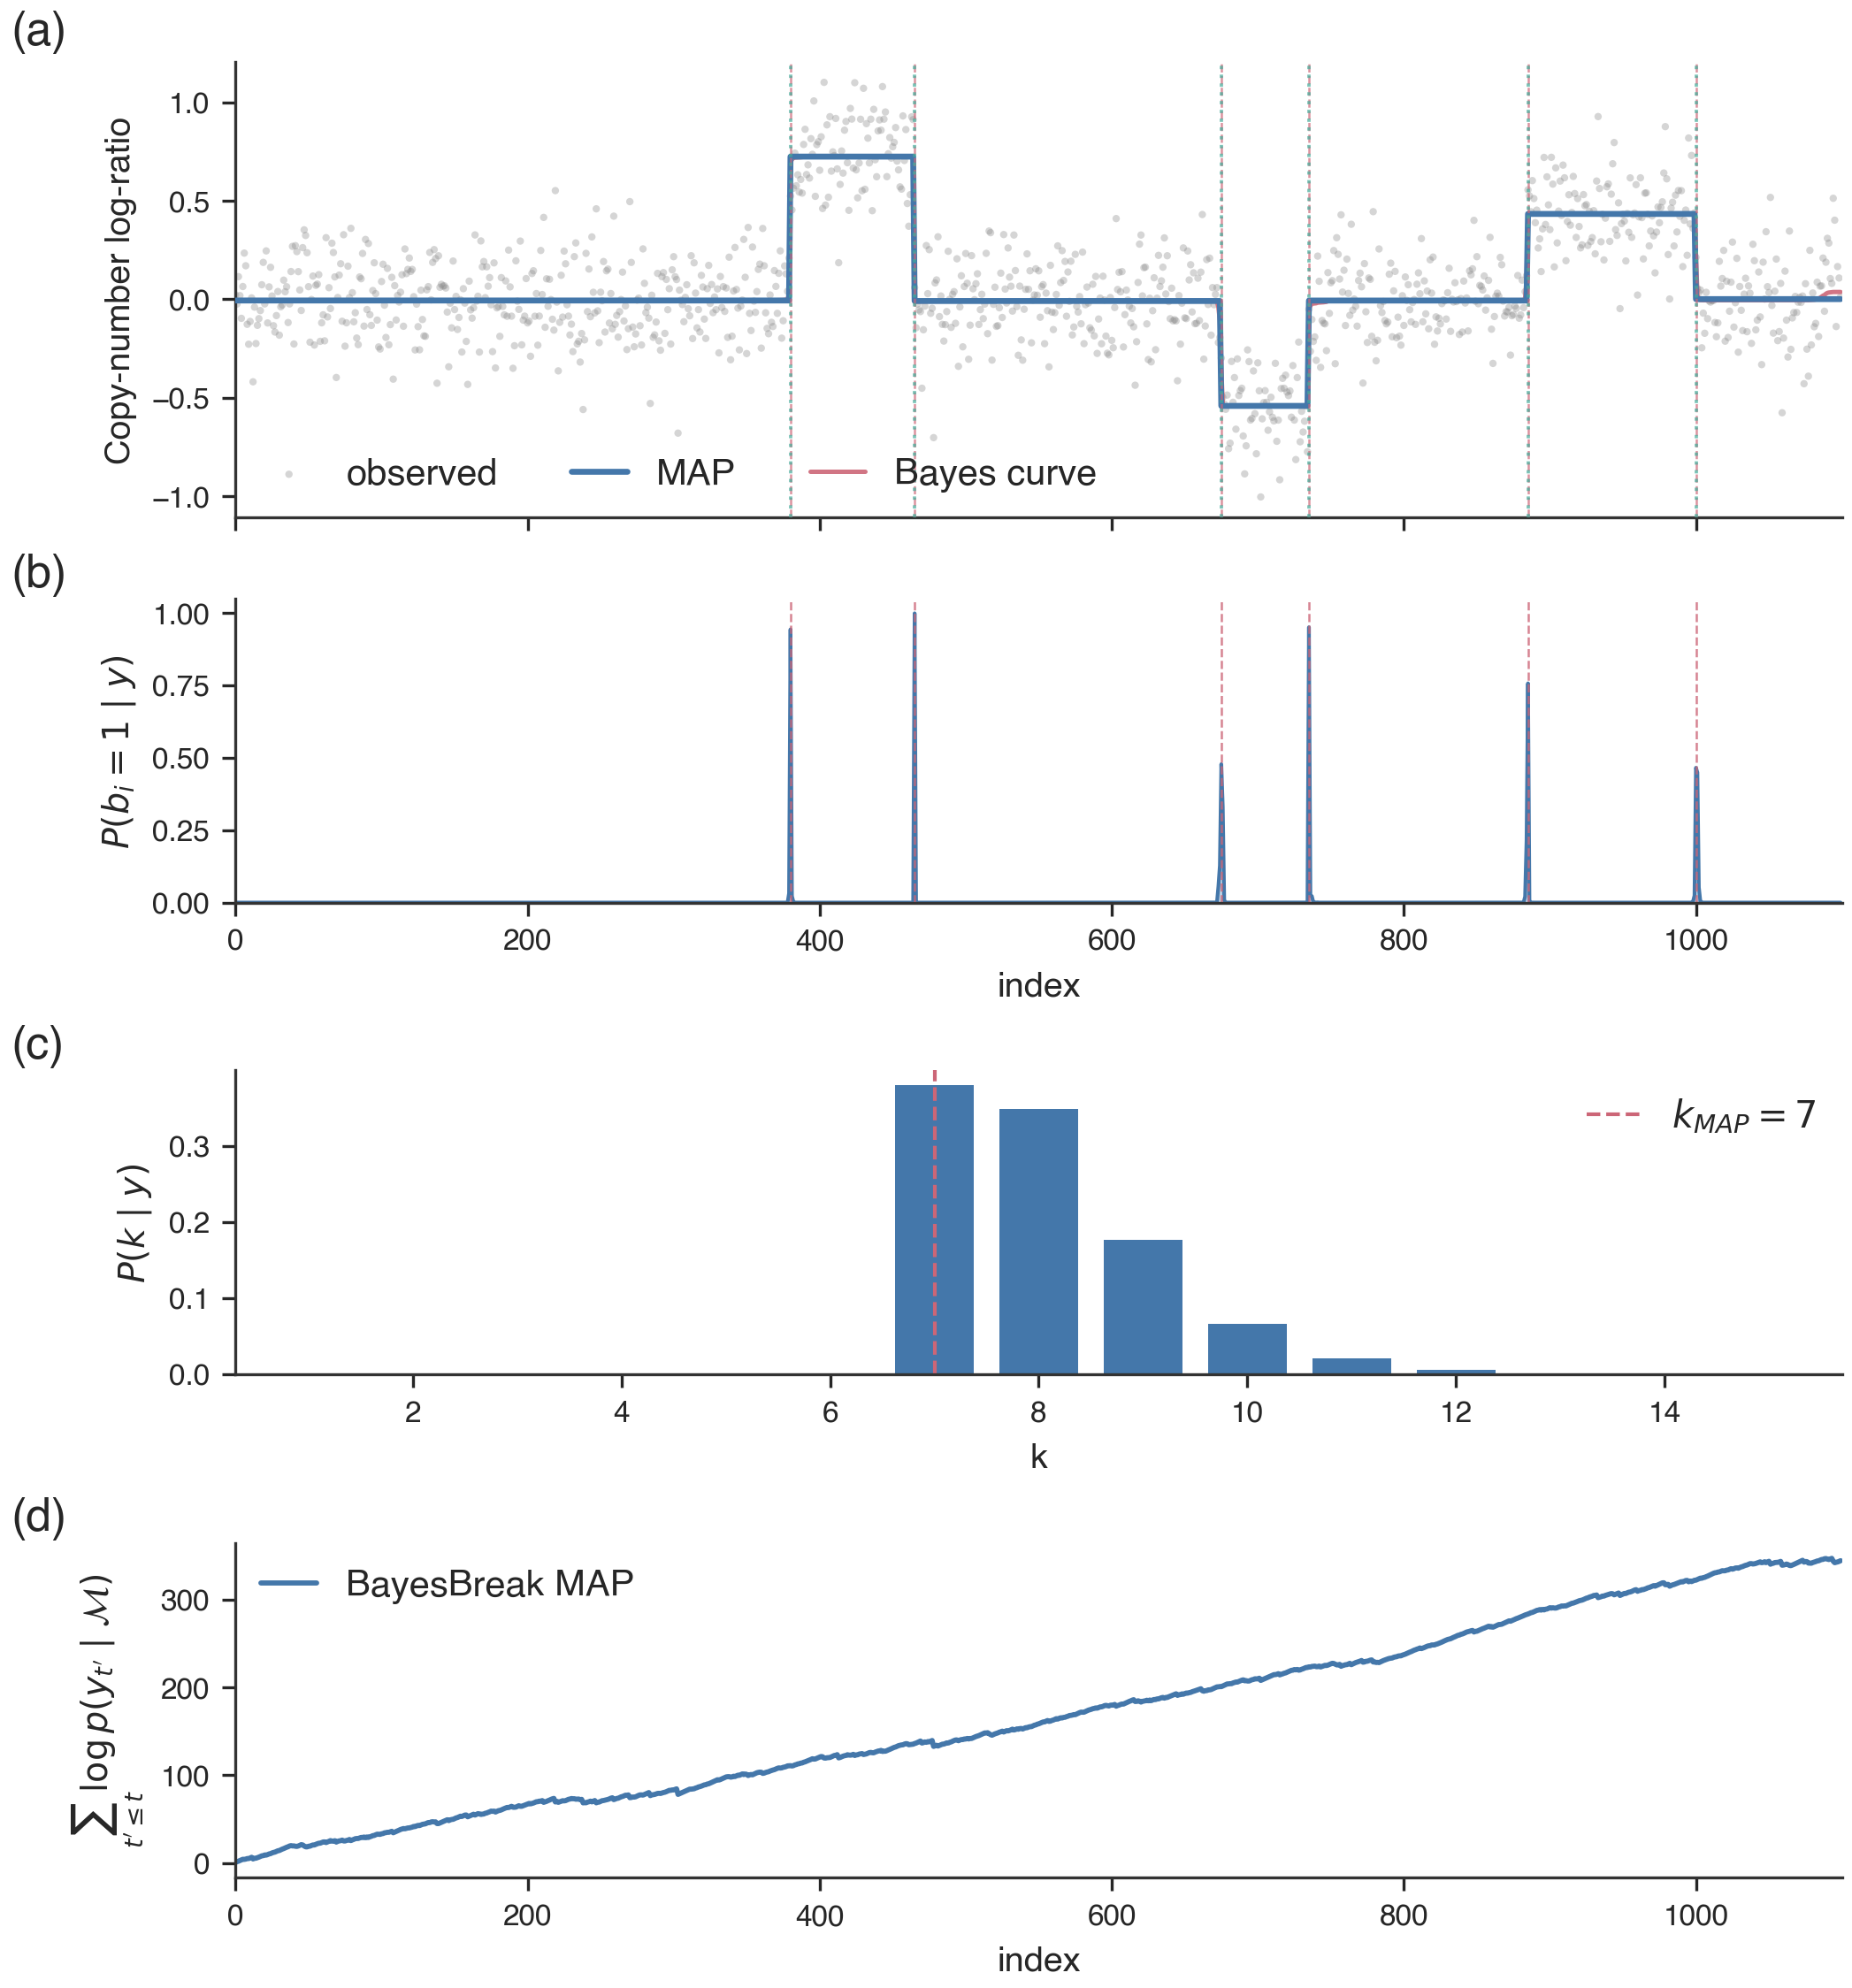
\includegraphics[width=0.90\textwidth,height=0.43\textheight,keepaspectratio]{figures/fig7_cgh.png}
  \caption{Shared-boundary array-CGH segmentation. The common red markers are
    fitted joint-MAP boundaries, not external copy-number annotations.}
  \label{fig:cgh-paper}
\end{figure}


\paragraph{S\&P 500.}
The S\&P 500 series was excluded from E09 because the \texttt{yfinance} package is not installed in the execution environment; \texttt{load\_spx()} returns a simulated fallback series. Per protocol, simulated data are never labeled as real observational data. No SPX result is reported from E09.

\paragraph{Methylation.}
The data are the \texttt{methylKit} \texttt{test1.myCpG} chromosome-21 example with 1,904 CpGs and per-CpG read coverage used as the Beta-observation precision $\phi_t$. Both the geometric and uniform count priors were persistently truncated at every tested $k_{\max}$ up to 120 ($P(k=120 \mid y) \approx 1.0$ for both priors at $k_{\max}=120$) (Figure~\ref{fig:methylation-paper}). The unrestricted MAP segment count is unknown; the high per-CpG read coverage makes even small methylation differences evidence for a changepoint, producing many short differential methylation regions. Extending $k_{\max}$ substantially beyond 120 is required to resolve the posterior.

No methylation atlas annotation was performed and no external boundary accuracy is reported.

\begin{figure}[!htbp]
  \centering
  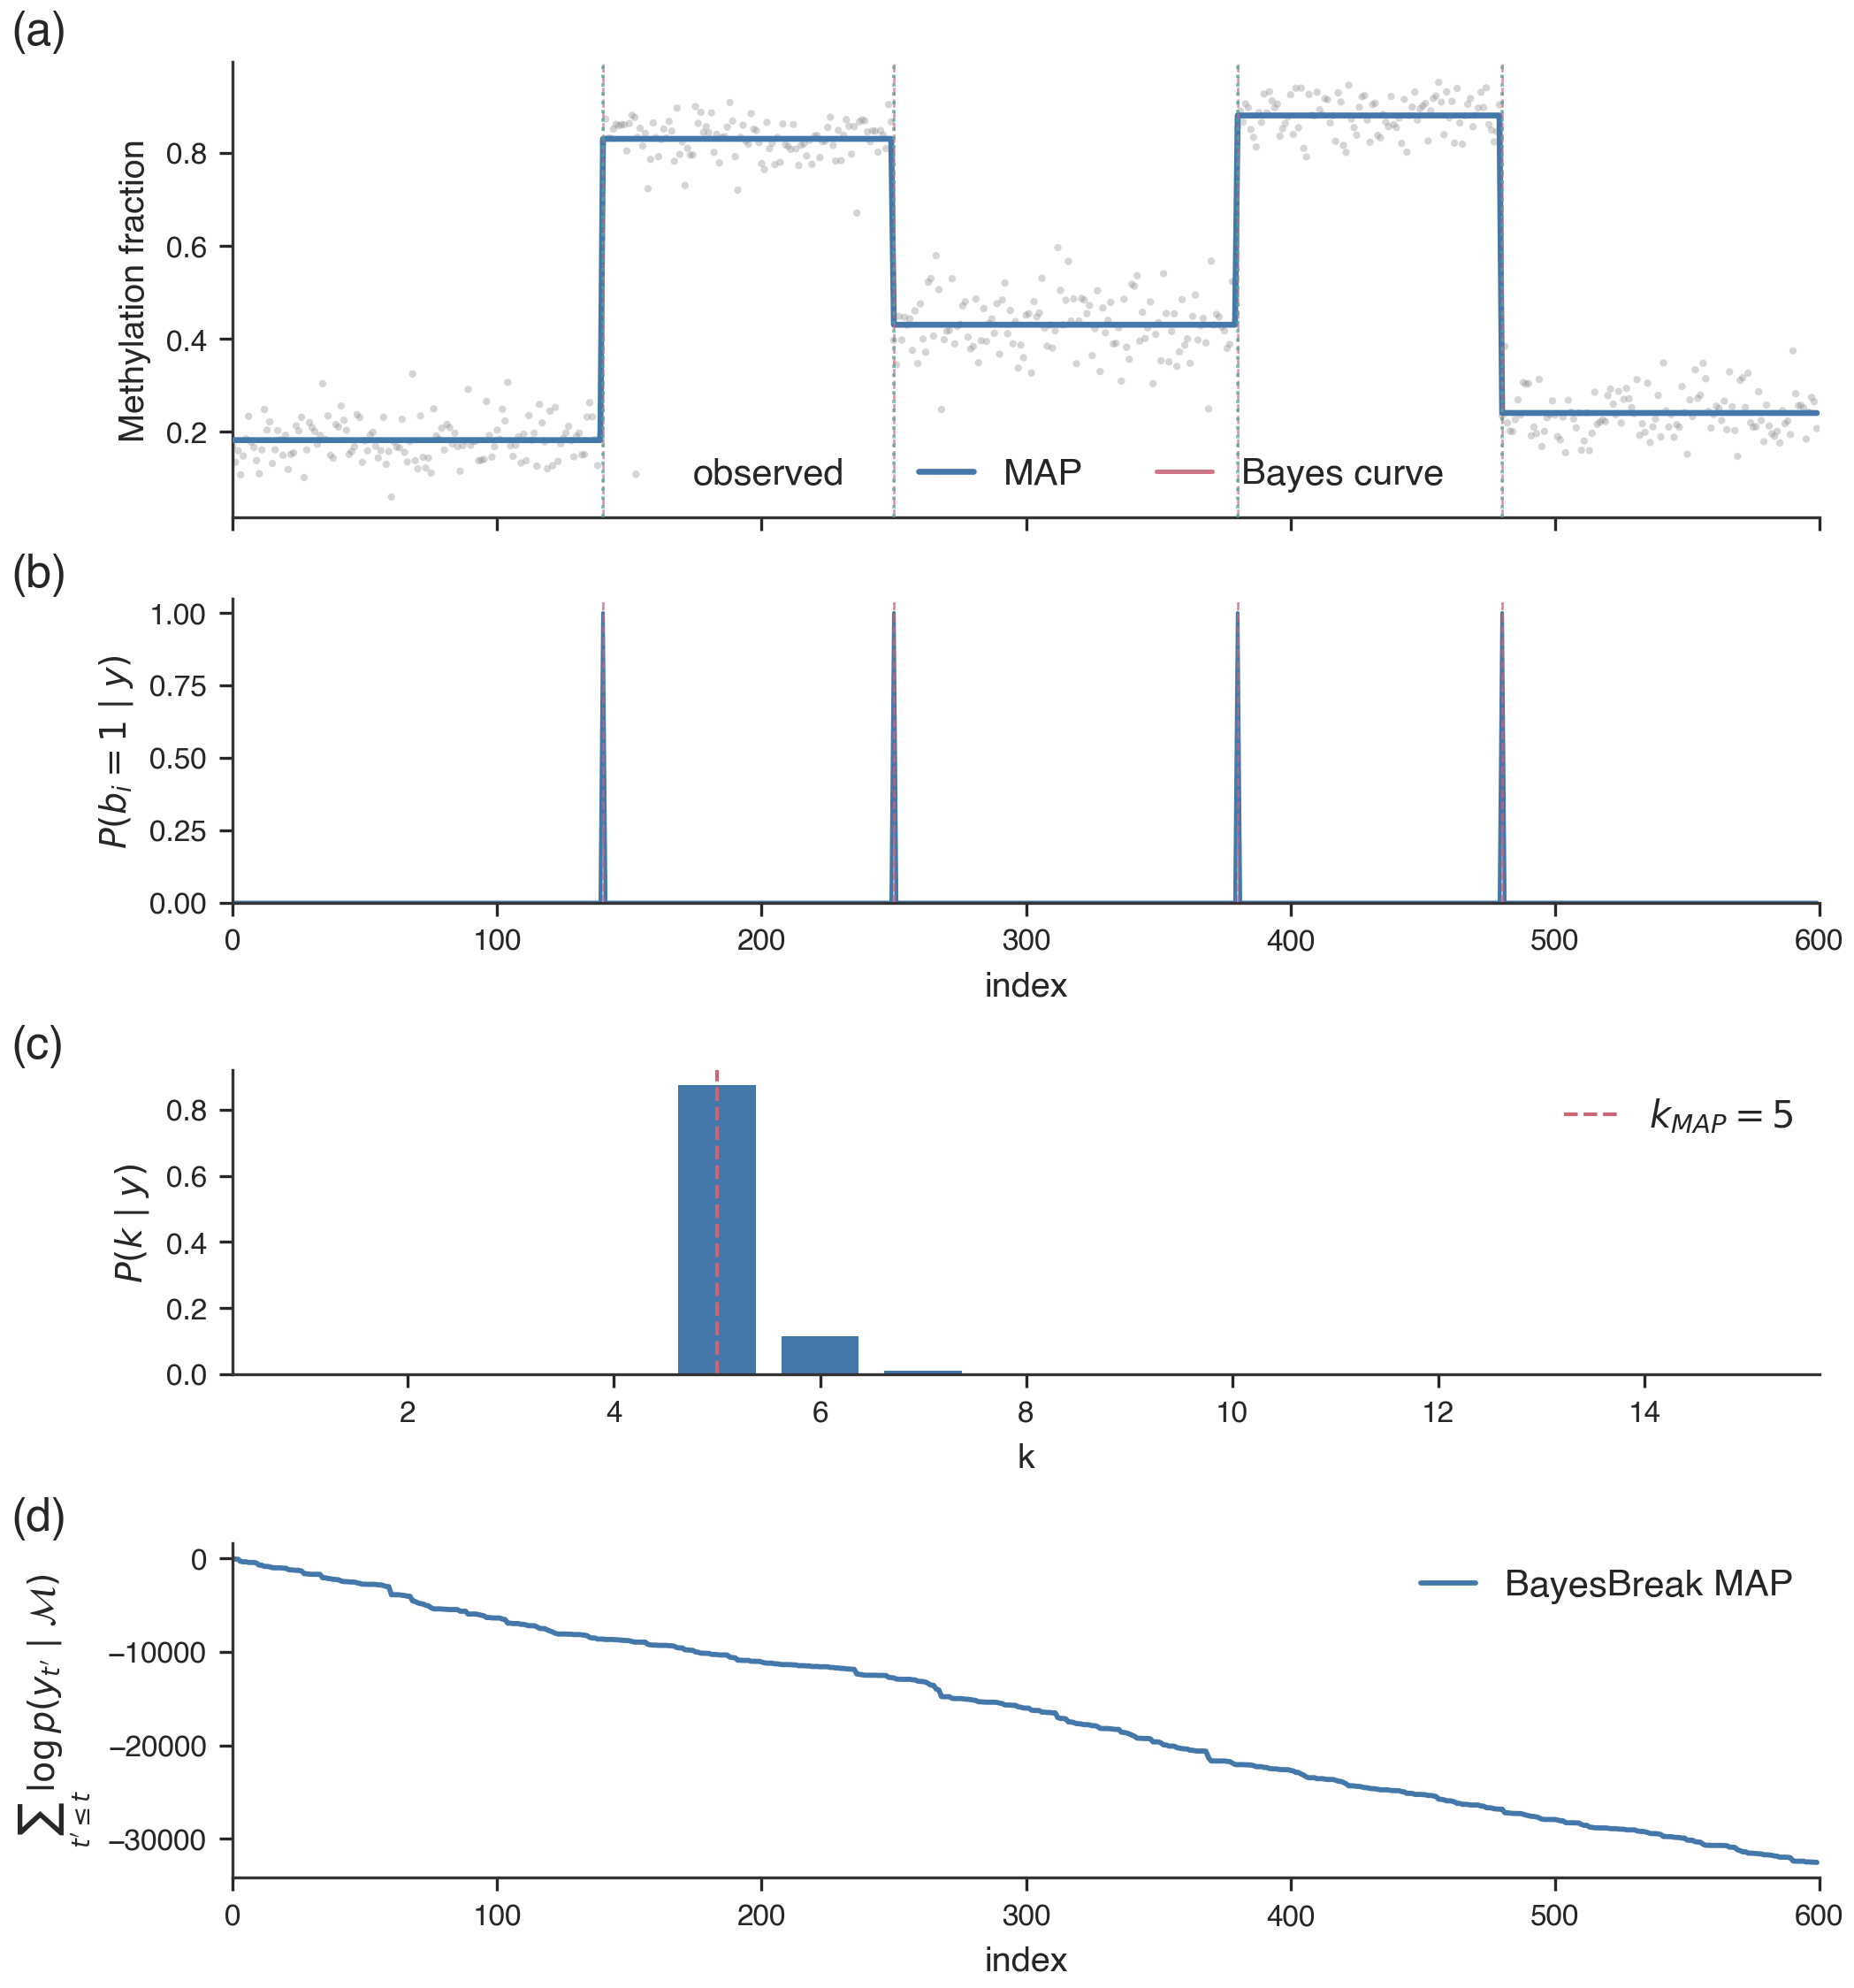
\includegraphics[width=0.90\textwidth,height=0.43\textheight,keepaspectratio]{figures/fig9_methylation.png}
  \caption{Beta-valued fit to the methylKit chromosome-21 example. Red markers are fitted
    MAP boundaries; no independent atlas transition annotation was used.}
  \label{fig:methylation-paper}
\end{figure}


\paragraph{E08 methylation predictive analysis.}
A separate posterior prediction evaluation (E08, artifact \texttt{a23d9fe92c02724c}) used the Beta-observation predictive distribution with observed held-out coverage as $\phi_{\mathrm{new}}$ and \texttt{extrapolation=error}. Ten disjoint stratified interior blocks held out 1,520 CpGs while retaining both fitted-support endpoints. Total log predictive score was $-23605.67$ and pooled mean score was $-15.53$ per held-out observation; the mean split score had a 95\% $t$ interval $[-23.14, -7.92]$. Mean boundary-stability $F_1@3$ against the full-data MAP was $0.879$. The blocks are regions of one chromosome, not independent biological samples. No certified PIT or external atlas accuracy is reported for this analysis.

\begin{figure}[!htbp]
  \centering
  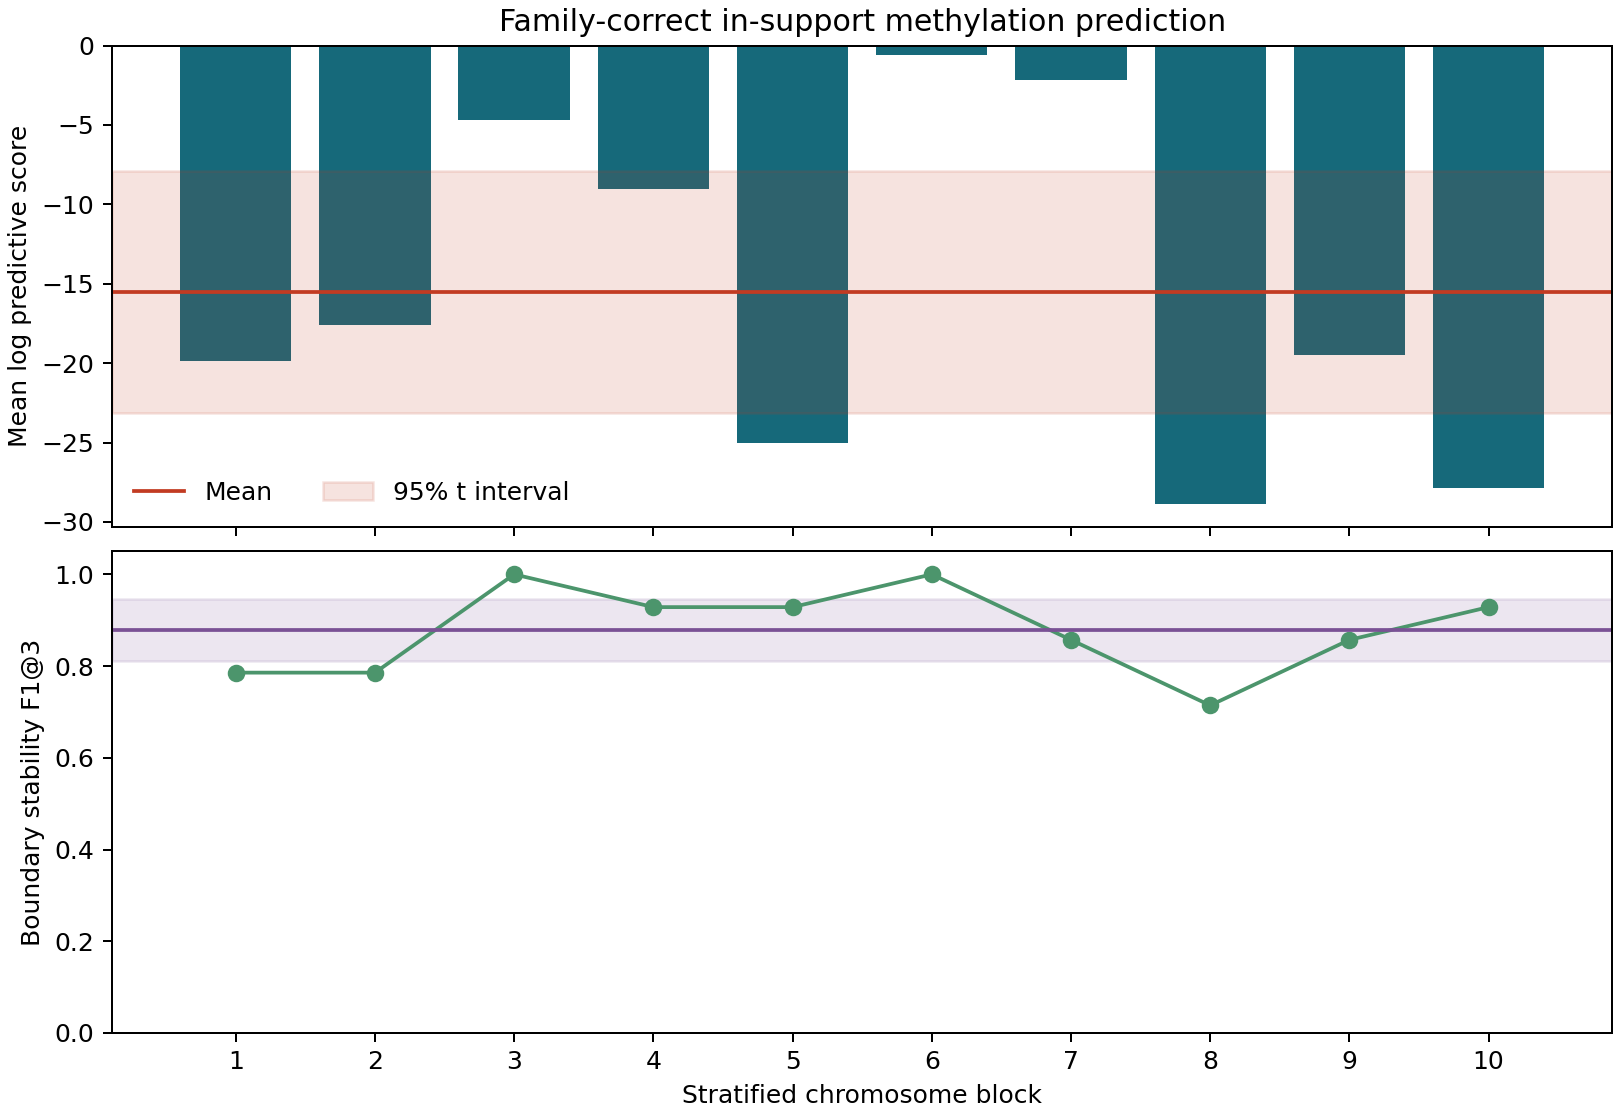
\includegraphics[width=0.86\textwidth,height=0.41\textheight,keepaspectratio]{figures/fig_methylation_heldout.png}
  \caption{Beta-response held-out prediction. Top: mean Beta-observation log predictive score
    across ten in-support chromosome blocks. Bottom: boundary-stability $F_1@3$ against
    the model-derived full-data MAP. Shaded bands are split-level 95\% $t$ intervals.}
  \label{fig:methyl-predictive-corrected-paper}
\end{figure}


\FloatBarrier
\subsection{Summary of empirical findings}
The empirical results confirm that common partition recursions can use closed-form conjugate segment marginal likelihoods, one-dimensional quadrature, other numerical segment calculations, shared-changepoint pooling, and finite latent-group templates. Experiment E00 verified the exact recursions and family-specific integrals by exhaustive partition enumeration ($n\in\{2,\ldots,10\}$, 4 families): all 380 oracle checks passed with boundary probability errors below $7.11\times10^{-15}$ and quadrature comparison errors below $3.91\times10^{-14}$ (artifact \texttt{03a4d1c38bfe08c1}). Experiment E01 provides pre-registered Gaussian calibration and recovery results across 22 cells at two sequence lengths ($n\in\{256,512\}$), with ECE below $0.0081$ in all strata and F1@3 above $0.93$ at strong signal ($\Delta/\sigma=2$); weak-signal undersegmentation is prior-induced, not a calibration property. Experiment E02 confirms mathematical portability of the exact inference pipeline across five declared exponential families (Gaussian, Poisson, Binomial, Negative Binomial, Beta-obs): F1@3 exceeded $0.88$ at the stronger effect setting in every family, with family-specific difficulty determined by observation variance and prior placement. Experiment E03 demonstrates that design-aware partition priors (gap hazard, length cohesion) correctly concentrate posterior probability at large-gap boundary locations when evidence supports a change, while preserving near-zero false-positive probability when it does not; F1@3 exceeded $0.85$ in all 24 cells. Experiment E04 confirms that exact common-boundary pooling accumulates information monotonically with $S$: pooled F1@3 reached $1.000$ for $S\geq16$ at full sharing while independent per-sequence fits remained near $0.893$; under complete boundary misspecification, the pooled model correctly degrades rather than silently producing invalid boundaries. Experiment E05 confirms that the template-mixture EM recovers latent group assignments correctly at moderate-to-strong signal ($\Delta\geq1.5$): ARI reached $1.000$ at $\Delta=1.5$ for $G\in\{2,3\}$; at weak signal ($\Delta=0.5$), group templates collapse and accuracy falls to near-chance levels; all 900 objective traces were non-decreasing. Experiment E06 benchmarked four block-evidence methods for the Bernoulli logistic-normal model on 1800 independently drawn blocks ($B\in\{4,8,16,32,64,128\}$, $p\in\{0.05,0.5,0.95\}$, 100 replicates per cell). Laplace approximation achieved median absolute log-evidence error $0.021$ and maximum $0.038$. JJ (Jaakkola--Jordan) is a rigorous variational lower bound: it produced zero violations of $\mathrm{JJ}\le\mathrm{reference}+10^{-8}$ across all 1800 blocks, with median error $0.222$ and maximum $0.977$. EP had median absolute error $3.779$ and maximum $30.001$, exceeding the quadrature reference in 1409 of 1800 blocks; EP is not a lower bound. In end-to-end segmentation propagation ($n=96$, $k_{\rm true}=3$, 100 replicates), Laplace caused 1 MAP mismatch of 100, JJ caused 19, and EP caused 89; mean $\mathrm{F}_1@3$ was $0.530$ for Laplace, $0.545$ for JJ, and $0.423$ for EP, versus $0.503$ for the quadrature reference. Experiment E07 evaluates robustness across 20 cells ($n=256$, $k_{\rm true}=3$, 100 replicates each): correct Gaussian specification achieved $\mathrm{F}_1@3=0.918$ with count exact-match $0.960$ at no missingness; MCAR 30\% and contiguous-block missingness reduced $\mathrm{F}_1@3$ to $0.809$ and $0.721$ respectively. Heavy-tail (Student-$t$) misspecification reduced $\mathrm{F}_1@3$ to $0.767$ and count accuracy to $0.530$ (extra segments absorb tail events). Fitting Poisson to overdispersed NegBin data gave $\mathrm{F}_1@3=0.525$ versus $0.709$ for the correct NegBin fit. Fitting Binomial to Beta-Binomial data gave the largest degradation: $\mathrm{F}_1@3=0.464$ and count exact-match $0.060$ (overdispersion overwhelmingly absorbed as extra segments). No numerical failures occurred across all 2000 replicates. Experiment E09 applied BayesBreak to four real datasets under the E09 protocol (artifact \texttt{0f5281c46ee8976e}): well-log (4050 NMR values, geometric prior, $\hat{k}=83$, resolved), array-CGH subject 0 (2215 probes, $\hat{k}=71$, resolved; pooled 43-subject fit truncated at $k_{\max}=60$), methylation (1904 CpGs, truncated at $k_{\max}=120$ under both priors), and S\&P 500 (excluded; \texttt{yfinance} unavailable in the execution environment). Twenty-five of 31 cells were truncated; the unrestricted MAP segment count is unknown for those fits. Experiment E10 benchmarked memory and runtime from $n=128$ to $n=2048$ at $k_{\max}=20$ across 15 cells: memory peaked at 500 MB at $n=2048$ with log-log slope converging to 2.0, consistent with $O(n^2)$ storage; forward-backward runtime had log-log slope $1.10$--$1.24$ in $n$; end-to-end runtime was $3.25$ seconds at $n=2048$, $k_{\max}=20$. These results do not establish external boundary accuracy, dominance under independently tuned predictive comparisons, routine-wide approximation guarantees, or asymptotic speed better than the quadratic dynamic-programming bound.
